\documentclass[b5paper,chapter,figtabcapt]{oblivoir}
\usepackage{graphicx}
\graphicspath{{imgs/}}
\chapterstyle{bianchi}
\renewcommand{\chaptitlefont}{\normalfont\huge\bfseries}
\hypersetup{
    %colorlinks=true,
    %linkcolor=blue,
    %filecolor=magenta,
    %urlcolor=cyan,
    %citecolor=olive,
    pdftitle={프로그래밍언어론},
    %pdfpagemode=FullScreen,
    }
\urlstyle{same}
%\usepackage[style=apa,natbib=true]{biblatex}
\usepackage[style=numeric-comp,natbib=true,sorting=nyt]{biblatex}
\addbibresource{sample.bib}
\usepackage{stmaryrd}
\usepackage{mathtools}
\usepackage{semantic}
\usepackage[linguistics]{forest}
\usepackage[hang]{caption}
\usepackage{subcaption}
\usepackage{listings}
\lstset{
    basicstyle=\ttfamily,
    basewidth={.5em}
}
\usepackage{float}

\usepackage{lipsum}

%%%%%%%% BEGIN: Jupyter generated LaTeX header %%%%%%%%
    \usepackage[breakable]{tcolorbox}
    \usepackage{parskip} % Stop auto-indenting (to mimic markdown behaviour)

    \usepackage{iftex}
    \ifPDFTeX
    	\usepackage[T1]{fontenc}
    	\usepackage{mathpazo}
    \else
    	\usepackage{fontspec}
    \fi

    % Basic figure setup, for now with no caption control since it's done
    % automatically by Pandoc (which extracts ![](path) syntax from Markdown).
    %% \usepackage{graphicx}
    %% Maintain compatibility with old templates. Remove in nbconvert 6.0
    %% \let\Oldincludegraphics\includegraphics
    %% % Ensure that by default, figures have no caption (until we provide a
    %% % proper Figure object with a Caption API and a way to capture that
    %% % in the conversion process - todo).
    %% \usepackage{caption}
    %% \DeclareCaptionFormat{nocaption}{}
    %% \captionsetup{format=nocaption,aboveskip=0pt,belowskip=0pt}

    %% \usepackage{float}
    %% \floatplacement{figure}{H} % forces figures to be placed at the correct location
    \usepackage{xcolor} % Allow colors to be defined
    \usepackage{enumerate} % Needed for markdown enumerations to work
    %% \usepackage{geometry} % Used to adjust the document margins
    \usepackage{amsmath} % Equations
    \usepackage{amssymb} % Equations
    \usepackage{textcomp} % defines textquotesingle
    % Hack from http://tex.stackexchange.com/a/47451/13684:
    \AtBeginDocument{%
        \def\PYZsq{\textquotesingle}% Upright quotes in Pygmentized code
    }
    \usepackage{upquote} % Upright quotes for verbatim code
    \usepackage{eurosym} % defines \euro
    %% \usepackage[mathletters]{ucs} % Extended unicode (utf-8) support
    \usepackage{fancyvrb} % verbatim replacement that allows latex
    \usepackage{grffile} % extends the file name processing of package graphics
                         % to support a larger range
    \makeatletter % fix for old versions of grffile with XeLaTeX
    \@ifpackagelater{grffile}{2019/11/01}
    {
      % Do nothing on new versions
    }
    {
      \def\Gread@@xetex#1{%
        \IfFileExists{"\Gin@base".bb}%
        {\Gread@eps{\Gin@base.bb}}%
        {\Gread@@xetex@aux#1}%
      }
    }
    \makeatother
    \usepackage[Export]{adjustbox} % Used to constrain images to a maximum size
    \adjustboxset{max size={0.9\linewidth}{0.9\paperheight}}

    % The default LaTeX title has an obnoxious amount of whitespace. By default,
    % titling removes some of it. It also provides customization options.
    \usepackage{titling}
    \usepackage{longtable} % longtable support required by pandoc >1.10
    \usepackage{booktabs}  % table support for pandoc > 1.12.2
    \usepackage[inline]{enumitem} % IRkernel/repr support (it uses the enumerate* environment)
    \usepackage[normalem]{ulem} % ulem is needed to support strikethroughs (\sout)
                                % normalem makes italics be italics, not underlines
    \usepackage{mathrsfs}



    % Colors for the hyperref package
    \definecolor{urlcolor}{rgb}{0,.145,.698}
    \definecolor{linkcolor}{rgb}{.71,0.21,0.01}
    \definecolor{citecolor}{rgb}{.12,.54,.11}

    % ANSI colors
    \definecolor{ansi-black}{HTML}{3E424D}
    \definecolor{ansi-black-intense}{HTML}{282C36}
    \definecolor{ansi-red}{HTML}{E75C58}
    \definecolor{ansi-red-intense}{HTML}{B22B31}
    \definecolor{ansi-green}{HTML}{00A250}
    \definecolor{ansi-green-intense}{HTML}{007427}
    \definecolor{ansi-yellow}{HTML}{DDB62B}
    \definecolor{ansi-yellow-intense}{HTML}{B27D12}
    \definecolor{ansi-blue}{HTML}{208FFB}
    \definecolor{ansi-blue-intense}{HTML}{0065CA}
    \definecolor{ansi-magenta}{HTML}{D160C4}
    \definecolor{ansi-magenta-intense}{HTML}{A03196}
    \definecolor{ansi-cyan}{HTML}{60C6C8}
    \definecolor{ansi-cyan-intense}{HTML}{258F8F}
    \definecolor{ansi-white}{HTML}{C5C1B4}
    \definecolor{ansi-white-intense}{HTML}{A1A6B2}
    \definecolor{ansi-default-inverse-fg}{HTML}{FFFFFF}
    \definecolor{ansi-default-inverse-bg}{HTML}{000000}

    % common color for the border for error outputs.
    \definecolor{outerrorbackground}{HTML}{FFDFDF}

    % commands and environments needed by pandoc snippets
    % extracted from the output of `pandoc -s`
    \providecommand{\tightlist}{%
      \setlength{\itemsep}{0pt}\setlength{\parskip}{0pt}}
    \DefineVerbatimEnvironment{Highlighting}{Verbatim}{commandchars=\\\{\}}
    % Add ',fontsize=\small' for more characters per line
    \newenvironment{Shaded}{}{}
    \newcommand{\KeywordTok}[1]{\textcolor[rgb]{0.00,0.44,0.13}{\textbf{{#1}}}}
    \newcommand{\DataTypeTok}[1]{\textcolor[rgb]{0.56,0.13,0.00}{{#1}}}
    \newcommand{\DecValTok}[1]{\textcolor[rgb]{0.25,0.63,0.44}{{#1}}}
    \newcommand{\BaseNTok}[1]{\textcolor[rgb]{0.25,0.63,0.44}{{#1}}}
    \newcommand{\FloatTok}[1]{\textcolor[rgb]{0.25,0.63,0.44}{{#1}}}
    \newcommand{\CharTok}[1]{\textcolor[rgb]{0.25,0.44,0.63}{{#1}}}
    \newcommand{\StringTok}[1]{\textcolor[rgb]{0.25,0.44,0.63}{{#1}}}
    \newcommand{\CommentTok}[1]{\textcolor[rgb]{0.38,0.63,0.69}{\textit{{#1}}}}
    \newcommand{\OtherTok}[1]{\textcolor[rgb]{0.00,0.44,0.13}{{#1}}}
    \newcommand{\AlertTok}[1]{\textcolor[rgb]{1.00,0.00,0.00}{\textbf{{#1}}}}
    \newcommand{\FunctionTok}[1]{\textcolor[rgb]{0.02,0.16,0.49}{{#1}}}
    \newcommand{\RegionMarkerTok}[1]{{#1}}
    \newcommand{\ErrorTok}[1]{\textcolor[rgb]{1.00,0.00,0.00}{\textbf{{#1}}}}
    \newcommand{\NormalTok}[1]{{#1}}

    % Additional commands for more recent versions of Pandoc
    \newcommand{\ConstantTok}[1]{\textcolor[rgb]{0.53,0.00,0.00}{{#1}}}
    \newcommand{\SpecialCharTok}[1]{\textcolor[rgb]{0.25,0.44,0.63}{{#1}}}
    \newcommand{\VerbatimStringTok}[1]{\textcolor[rgb]{0.25,0.44,0.63}{{#1}}}
    \newcommand{\SpecialStringTok}[1]{\textcolor[rgb]{0.73,0.40,0.53}{{#1}}}
    \newcommand{\ImportTok}[1]{{#1}}
    \newcommand{\DocumentationTok}[1]{\textcolor[rgb]{0.73,0.13,0.13}{\textit{{#1}}}}
    \newcommand{\AnnotationTok}[1]{\textcolor[rgb]{0.38,0.63,0.69}{\textbf{\textit{{#1}}}}}
    \newcommand{\CommentVarTok}[1]{\textcolor[rgb]{0.38,0.63,0.69}{\textbf{\textit{{#1}}}}}
    \newcommand{\VariableTok}[1]{\textcolor[rgb]{0.10,0.09,0.49}{{#1}}}
    \newcommand{\ControlFlowTok}[1]{\textcolor[rgb]{0.00,0.44,0.13}{\textbf{{#1}}}}
    \newcommand{\OperatorTok}[1]{\textcolor[rgb]{0.40,0.40,0.40}{{#1}}}
    \newcommand{\BuiltInTok}[1]{{#1}}
    \newcommand{\ExtensionTok}[1]{{#1}}
    \newcommand{\PreprocessorTok}[1]{\textcolor[rgb]{0.74,0.48,0.00}{{#1}}}
    \newcommand{\AttributeTok}[1]{\textcolor[rgb]{0.49,0.56,0.16}{{#1}}}
    \newcommand{\InformationTok}[1]{\textcolor[rgb]{0.38,0.63,0.69}{\textbf{\textit{{#1}}}}}
    \newcommand{\WarningTok}[1]{\textcolor[rgb]{0.38,0.63,0.69}{\textbf{\textit{{#1}}}}}


    % Define a nice break command that doesn't care if a line doesn't already
    % exist.
    \def\br{\hspace*{\fill} \\* }
    % Math Jax compatibility definitions
    \def\gt{>}
    \def\lt{<}
    \let\Oldtex\TeX
    \let\Oldlatex\LaTeX
    \renewcommand{\TeX}{\textrm{\Oldtex}}
    \renewcommand{\LaTeX}{\textrm{\Oldlatex}}
    % Document parameters
    % Document title
    \title{Untitled}





% Pygments definitions
\makeatletter
\def\PY@reset{\let\PY@it=\relax \let\PY@bf=\relax%
    \let\PY@ul=\relax \let\PY@tc=\relax%
    \let\PY@bc=\relax \let\PY@ff=\relax}
\def\PY@tok#1{\csname PY@tok@#1\endcsname}
\def\PY@toks#1+{\ifx\relax#1\empty\else%
    \PY@tok{#1}\expandafter\PY@toks\fi}
\def\PY@do#1{\PY@bc{\PY@tc{\PY@ul{%
    \PY@it{\PY@bf{\PY@ff{#1}}}}}}}
\def\PY#1#2{\PY@reset\PY@toks#1+\relax+\PY@do{#2}}

\@namedef{PY@tok@w}{\def\PY@tc##1{\textcolor[rgb]{0.73,0.73,0.73}{##1}}}
\@namedef{PY@tok@c}{\let\PY@it=\textit\def\PY@tc##1{\textcolor[rgb]{0.25,0.50,0.50}{##1}}}
\@namedef{PY@tok@cp}{\def\PY@tc##1{\textcolor[rgb]{0.74,0.48,0.00}{##1}}}
\@namedef{PY@tok@k}{\let\PY@bf=\textbf\def\PY@tc##1{\textcolor[rgb]{0.00,0.50,0.00}{##1}}}
\@namedef{PY@tok@kp}{\def\PY@tc##1{\textcolor[rgb]{0.00,0.50,0.00}{##1}}}
\@namedef{PY@tok@kt}{\def\PY@tc##1{\textcolor[rgb]{0.69,0.00,0.25}{##1}}}
\@namedef{PY@tok@o}{\def\PY@tc##1{\textcolor[rgb]{0.40,0.40,0.40}{##1}}}
\@namedef{PY@tok@ow}{\let\PY@bf=\textbf\def\PY@tc##1{\textcolor[rgb]{0.67,0.13,1.00}{##1}}}
\@namedef{PY@tok@nb}{\def\PY@tc##1{\textcolor[rgb]{0.00,0.50,0.00}{##1}}}
\@namedef{PY@tok@nf}{\def\PY@tc##1{\textcolor[rgb]{0.00,0.00,1.00}{##1}}}
\@namedef{PY@tok@nc}{\let\PY@bf=\textbf\def\PY@tc##1{\textcolor[rgb]{0.00,0.00,1.00}{##1}}}
\@namedef{PY@tok@nn}{\let\PY@bf=\textbf\def\PY@tc##1{\textcolor[rgb]{0.00,0.00,1.00}{##1}}}
\@namedef{PY@tok@ne}{\let\PY@bf=\textbf\def\PY@tc##1{\textcolor[rgb]{0.82,0.25,0.23}{##1}}}
\@namedef{PY@tok@nv}{\def\PY@tc##1{\textcolor[rgb]{0.10,0.09,0.49}{##1}}}
\@namedef{PY@tok@no}{\def\PY@tc##1{\textcolor[rgb]{0.53,0.00,0.00}{##1}}}
\@namedef{PY@tok@nl}{\def\PY@tc##1{\textcolor[rgb]{0.63,0.63,0.00}{##1}}}
\@namedef{PY@tok@ni}{\let\PY@bf=\textbf\def\PY@tc##1{\textcolor[rgb]{0.60,0.60,0.60}{##1}}}
\@namedef{PY@tok@na}{\def\PY@tc##1{\textcolor[rgb]{0.49,0.56,0.16}{##1}}}
\@namedef{PY@tok@nt}{\let\PY@bf=\textbf\def\PY@tc##1{\textcolor[rgb]{0.00,0.50,0.00}{##1}}}
\@namedef{PY@tok@nd}{\def\PY@tc##1{\textcolor[rgb]{0.67,0.13,1.00}{##1}}}
\@namedef{PY@tok@s}{\def\PY@tc##1{\textcolor[rgb]{0.73,0.13,0.13}{##1}}}
\@namedef{PY@tok@sd}{\let\PY@it=\textit\def\PY@tc##1{\textcolor[rgb]{0.73,0.13,0.13}{##1}}}
\@namedef{PY@tok@si}{\let\PY@bf=\textbf\def\PY@tc##1{\textcolor[rgb]{0.73,0.40,0.53}{##1}}}
\@namedef{PY@tok@se}{\let\PY@bf=\textbf\def\PY@tc##1{\textcolor[rgb]{0.73,0.40,0.13}{##1}}}
\@namedef{PY@tok@sr}{\def\PY@tc##1{\textcolor[rgb]{0.73,0.40,0.53}{##1}}}
\@namedef{PY@tok@ss}{\def\PY@tc##1{\textcolor[rgb]{0.10,0.09,0.49}{##1}}}
\@namedef{PY@tok@sx}{\def\PY@tc##1{\textcolor[rgb]{0.00,0.50,0.00}{##1}}}
\@namedef{PY@tok@m}{\def\PY@tc##1{\textcolor[rgb]{0.40,0.40,0.40}{##1}}}
\@namedef{PY@tok@gh}{\let\PY@bf=\textbf\def\PY@tc##1{\textcolor[rgb]{0.00,0.00,0.50}{##1}}}
\@namedef{PY@tok@gu}{\let\PY@bf=\textbf\def\PY@tc##1{\textcolor[rgb]{0.50,0.00,0.50}{##1}}}
\@namedef{PY@tok@gd}{\def\PY@tc##1{\textcolor[rgb]{0.63,0.00,0.00}{##1}}}
\@namedef{PY@tok@gi}{\def\PY@tc##1{\textcolor[rgb]{0.00,0.63,0.00}{##1}}}
\@namedef{PY@tok@gr}{\def\PY@tc##1{\textcolor[rgb]{1.00,0.00,0.00}{##1}}}
\@namedef{PY@tok@ge}{\let\PY@it=\textit}
\@namedef{PY@tok@gs}{\let\PY@bf=\textbf}
\@namedef{PY@tok@gp}{\let\PY@bf=\textbf\def\PY@tc##1{\textcolor[rgb]{0.00,0.00,0.50}{##1}}}
\@namedef{PY@tok@go}{\def\PY@tc##1{\textcolor[rgb]{0.53,0.53,0.53}{##1}}}
\@namedef{PY@tok@gt}{\def\PY@tc##1{\textcolor[rgb]{0.00,0.27,0.87}{##1}}}
\@namedef{PY@tok@err}{\def\PY@bc##1{{\setlength{\fboxsep}{\string -\fboxrule}\fcolorbox[rgb]{1.00,0.00,0.00}{1,1,1}{\strut ##1}}}}
\@namedef{PY@tok@kc}{\let\PY@bf=\textbf\def\PY@tc##1{\textcolor[rgb]{0.00,0.50,0.00}{##1}}}
\@namedef{PY@tok@kd}{\let\PY@bf=\textbf\def\PY@tc##1{\textcolor[rgb]{0.00,0.50,0.00}{##1}}}
\@namedef{PY@tok@kn}{\let\PY@bf=\textbf\def\PY@tc##1{\textcolor[rgb]{0.00,0.50,0.00}{##1}}}
\@namedef{PY@tok@kr}{\let\PY@bf=\textbf\def\PY@tc##1{\textcolor[rgb]{0.00,0.50,0.00}{##1}}}
\@namedef{PY@tok@bp}{\def\PY@tc##1{\textcolor[rgb]{0.00,0.50,0.00}{##1}}}
\@namedef{PY@tok@fm}{\def\PY@tc##1{\textcolor[rgb]{0.00,0.00,1.00}{##1}}}
\@namedef{PY@tok@vc}{\def\PY@tc##1{\textcolor[rgb]{0.10,0.09,0.49}{##1}}}
\@namedef{PY@tok@vg}{\def\PY@tc##1{\textcolor[rgb]{0.10,0.09,0.49}{##1}}}
\@namedef{PY@tok@vi}{\def\PY@tc##1{\textcolor[rgb]{0.10,0.09,0.49}{##1}}}
\@namedef{PY@tok@vm}{\def\PY@tc##1{\textcolor[rgb]{0.10,0.09,0.49}{##1}}}
\@namedef{PY@tok@sa}{\def\PY@tc##1{\textcolor[rgb]{0.73,0.13,0.13}{##1}}}
\@namedef{PY@tok@sb}{\def\PY@tc##1{\textcolor[rgb]{0.73,0.13,0.13}{##1}}}
\@namedef{PY@tok@sc}{\def\PY@tc##1{\textcolor[rgb]{0.73,0.13,0.13}{##1}}}
\@namedef{PY@tok@dl}{\def\PY@tc##1{\textcolor[rgb]{0.73,0.13,0.13}{##1}}}
\@namedef{PY@tok@s2}{\def\PY@tc##1{\textcolor[rgb]{0.73,0.13,0.13}{##1}}}
\@namedef{PY@tok@sh}{\def\PY@tc##1{\textcolor[rgb]{0.73,0.13,0.13}{##1}}}
\@namedef{PY@tok@s1}{\def\PY@tc##1{\textcolor[rgb]{0.73,0.13,0.13}{##1}}}
\@namedef{PY@tok@mb}{\def\PY@tc##1{\textcolor[rgb]{0.40,0.40,0.40}{##1}}}
\@namedef{PY@tok@mf}{\def\PY@tc##1{\textcolor[rgb]{0.40,0.40,0.40}{##1}}}
\@namedef{PY@tok@mh}{\def\PY@tc##1{\textcolor[rgb]{0.40,0.40,0.40}{##1}}}
\@namedef{PY@tok@mi}{\def\PY@tc##1{\textcolor[rgb]{0.40,0.40,0.40}{##1}}}
\@namedef{PY@tok@il}{\def\PY@tc##1{\textcolor[rgb]{0.40,0.40,0.40}{##1}}}
\@namedef{PY@tok@mo}{\def\PY@tc##1{\textcolor[rgb]{0.40,0.40,0.40}{##1}}}
\@namedef{PY@tok@ch}{\let\PY@it=\textit\def\PY@tc##1{\textcolor[rgb]{0.25,0.50,0.50}{##1}}}
\@namedef{PY@tok@cm}{\let\PY@it=\textit\def\PY@tc##1{\textcolor[rgb]{0.25,0.50,0.50}{##1}}}
\@namedef{PY@tok@cpf}{\let\PY@it=\textit\def\PY@tc##1{\textcolor[rgb]{0.25,0.50,0.50}{##1}}}
\@namedef{PY@tok@c1}{\let\PY@it=\textit\def\PY@tc##1{\textcolor[rgb]{0.25,0.50,0.50}{##1}}}
\@namedef{PY@tok@cs}{\let\PY@it=\textit\def\PY@tc##1{\textcolor[rgb]{0.25,0.50,0.50}{##1}}}

\def\PYZbs{\char`\\}
\def\PYZus{\char`\_}
\def\PYZob{\char`\{}
\def\PYZcb{\char`\}}
\def\PYZca{\char`\^}
\def\PYZam{\char`\&}
\def\PYZlt{\char`\<}
\def\PYZgt{\char`\>}
\def\PYZsh{\char`\#}
\def\PYZpc{\char`\%}
\def\PYZdl{\char`\$}
\def\PYZhy{\char`\-}
\def\PYZsq{\char`\'}
\def\PYZdq{\char`\"}
\def\PYZti{\char`\~}
% for compatibility with earlier versions
\def\PYZat{@}
\def\PYZlb{[}
\def\PYZrb{]}
\makeatother


    % For linebreaks inside Verbatim environment from package fancyvrb.
    \makeatletter
        \newbox\Wrappedcontinuationbox
        \newbox\Wrappedvisiblespacebox
        \newcommand*\Wrappedvisiblespace {\textcolor{red}{\textvisiblespace}}
        \newcommand*\Wrappedcontinuationsymbol {\textcolor{red}{\llap{\tiny$\m@th\hookrightarrow$}}}
        \newcommand*\Wrappedcontinuationindent {3ex }
        \newcommand*\Wrappedafterbreak {\kern\Wrappedcontinuationindent\copy\Wrappedcontinuationbox}
        % Take advantage of the already applied Pygments mark-up to insert
        % potential linebreaks for TeX processing.
        %        {, <, #, %, $, ' and ": go to next line.
        %        _, }, ^, &, >, - and ~: stay at end of broken line.
        % Use of \textquotesingle for straight quote.
        \newcommand*\Wrappedbreaksatspecials {%
            \def\PYGZus{\discretionary{\char`\_}{\Wrappedafterbreak}{\char`\_}}%
            \def\PYGZob{\discretionary{}{\Wrappedafterbreak\char`\{}{\char`\{}}%
            \def\PYGZcb{\discretionary{\char`\}}{\Wrappedafterbreak}{\char`\}}}%
            \def\PYGZca{\discretionary{\char`\^}{\Wrappedafterbreak}{\char`\^}}%
            \def\PYGZam{\discretionary{\char`\&}{\Wrappedafterbreak}{\char`\&}}%
            \def\PYGZlt{\discretionary{}{\Wrappedafterbreak\char`\<}{\char`\<}}%
            \def\PYGZgt{\discretionary{\char`\>}{\Wrappedafterbreak}{\char`\>}}%
            \def\PYGZsh{\discretionary{}{\Wrappedafterbreak\char`\#}{\char`\#}}%
            \def\PYGZpc{\discretionary{}{\Wrappedafterbreak\char`\%}{\char`\%}}%
            \def\PYGZdl{\discretionary{}{\Wrappedafterbreak\char`\$}{\char`\$}}%
            \def\PYGZhy{\discretionary{\char`\-}{\Wrappedafterbreak}{\char`\-}}%
            \def\PYGZsq{\discretionary{}{\Wrappedafterbreak\textquotesingle}{\textquotesingle}}%
            \def\PYGZdq{\discretionary{}{\Wrappedafterbreak\char`\"}{\char`\"}}%
            \def\PYGZti{\discretionary{\char`\~}{\Wrappedafterbreak}{\char`\~}}%
        }
        % Some characters . , ; ? ! / are not pygmentized.
        % This macro makes them "active" and they will insert potential linebreaks
        \newcommand*\Wrappedbreaksatpunct {%
            \lccode`\~`\.\lowercase{\def~}{\discretionary{\hbox{\char`\.}}{\Wrappedafterbreak}{\hbox{\char`\.}}}%
            \lccode`\~`\,\lowercase{\def~}{\discretionary{\hbox{\char`\,}}{\Wrappedafterbreak}{\hbox{\char`\,}}}%
            \lccode`\~`\;\lowercase{\def~}{\discretionary{\hbox{\char`\;}}{\Wrappedafterbreak}{\hbox{\char`\;}}}%
            \lccode`\~`\:\lowercase{\def~}{\discretionary{\hbox{\char`\:}}{\Wrappedafterbreak}{\hbox{\char`\:}}}%
            \lccode`\~`\?\lowercase{\def~}{\discretionary{\hbox{\char`\?}}{\Wrappedafterbreak}{\hbox{\char`\?}}}%
            \lccode`\~`\!\lowercase{\def~}{\discretionary{\hbox{\char`\!}}{\Wrappedafterbreak}{\hbox{\char`\!}}}%
            \lccode`\~`\/\lowercase{\def~}{\discretionary{\hbox{\char`\/}}{\Wrappedafterbreak}{\hbox{\char`\/}}}%
            \catcode`\.\active
            \catcode`\,\active
            \catcode`\;\active
            \catcode`\:\active
            \catcode`\?\active
            \catcode`\!\active
            \catcode`\/\active
            \lccode`\~`\~
        }
    \makeatother

    \let\OriginalVerbatim=\Verbatim
    \makeatletter
    \renewcommand{\Verbatim}[1][1]{%
        %\parskip\z@skip
        \sbox\Wrappedcontinuationbox {\Wrappedcontinuationsymbol}%
        \sbox\Wrappedvisiblespacebox {\FV@SetupFont\Wrappedvisiblespace}%
        \def\FancyVerbFormatLine ##1{\hsize\linewidth
            \vtop{\raggedright\hyphenpenalty\z@\exhyphenpenalty\z@
                \doublehyphendemerits\z@\finalhyphendemerits\z@
                \strut ##1\strut}%
        }%
        % If the linebreak is at a space, the latter will be displayed as visible
        % space at end of first line, and a continuation symbol starts next line.
        % Stretch/shrink are however usually zero for typewriter font.
        \def\FV@Space {%
            \nobreak\hskip\z@ plus\fontdimen3\font minus\fontdimen4\font
            \discretionary{\copy\Wrappedvisiblespacebox}{\Wrappedafterbreak}
            {\kern\fontdimen2\font}%
        }%

        % Allow breaks at special characters using \PYG... macros.
        \Wrappedbreaksatspecials
        % Breaks at punctuation characters . , ; ? ! and / need catcode=\active
        \OriginalVerbatim[#1,codes*=\Wrappedbreaksatpunct]%
    }
    \makeatother

    % Exact colors from NB
    \definecolor{incolor}{HTML}{303F9F}
    \definecolor{outcolor}{HTML}{D84315}
    \definecolor{cellborder}{HTML}{CFCFCF}
    \definecolor{cellbackground}{HTML}{F7F7F7}

    % prompt
    \makeatletter
    \newcommand{\boxspacing}{\kern\kvtcb@left@rule\kern\kvtcb@boxsep}
    \makeatother
    \newcommand{\prompt}[4]{
        {\ttfamily\llap{{\color{#2}[#3]:\hspace{3pt}#4}}\vspace{-\baselineskip}}
    }



    % Prevent overflowing lines due to hard-to-break entities
    \sloppy
    % Setup hyperref package
    \hypersetup{
      breaklinks=true,  % so long urls are correctly broken across lines
      colorlinks=true,
      urlcolor=urlcolor,
      linkcolor=linkcolor,
      citecolor=citecolor,
      }
    %% % Slightly bigger margins than the latex defaults
    %%
    %% \geometry{verbose,tmargin=1in,bmargin=1in,lmargin=1in,rmargin=1in}

%%%%%%%% END:   Jupyter generated LaTeX header %%%%%%%%

\newcommand{\txtbullet}[0]{\ensuremath{\bullet}}
\newcommand{\txtcircle}[0]{\ensuremath{\circ}}

\newcommand{\VERT}{\ensuremath{\mathop{\!\resizebox{1.65ex}{.7em}{\texttt{|}}\!}}}

\title{프로그래밍언어론}
\author{안기영 \and 손범준}
%\date{2022-??-??}

\begin{document}

\maketitle

\frontmatter 

\chapter*{서문}
책을 쓰기 시작하면서 프로그래밍언어 분야의 용어가 얼마나 혼란스러울 수 있는지
다시금 돌아보는 계기가 되었다. 섬세하지 못한 번역이나 학계 용어 정리의 문제가
아니라 여러 기초 학문 분야가 관련되어 있어 용어/개념이 학문 분야의 경계를
넘나들며 맥락에 따라 의미의 차이가 발생할 수밖에 없는 측면이 있다. 첫 부분을
용어와 기본 개념에 대해 다루며 시작하는 것이 그런 이유에서다. 그리고
프로그래밍언어의 문법을 기술하고 분석하는 데 있어 형식언어에 대한 최소한의
이해가 있어야 하므로 관련된 기본 개념도 앞부분에서 짧은 분량으로나마
간략히 최소한의 개념을 소개하는 정도로 다루고 있다. 컴퓨터 관련
전공 과정이라 하더라도 응용 분야가 다양해지고 세분화되는 시대인 만큼
형식언어/오토마타/계산이론을 주제로 한 전공과목이 없는 경우도 있고
있다 하더라도 프로그래밍언어를 주제로 하는 강좌의 선수과목 혹은
저학년에 배치되지 않은 경우에도 한 교재 안에서 최소한의 내용을
참고할 수 있도록 하기 위함이다.

\newpage
\tableofcontents

\newpage
\listoffigures

\mainmatter

%%%%%%%%%%%%%%%%%%%%%%%%%%%%%%%%%%%%%%%%%%%%%%%%%%%%%%%%%%%%
\part{용어 및 기본 개념}
%%%%%%%%%%%%%%%%%%%%%%%%%%%%%%%%%%%%%%%%%%%%%%%%%%%%%%%%%%%%

\chapter{Syntax와 Grammar}
\label{chap:SyntaxGrammar}
똑같은 한글 글자로 된 우리말 단어를 접하더라도 각자의 배경에 따라
그 용어를 해석하는 바가 달라진다. `정의'를 영어로 뭐냐고 물어보았을 때
justice라고 대답하면 문과, definition이라고 대답하면 이과 출신이라는
고전 유머를 한번쯤 들어 보았을 것이다. 참고로,
justice를 뜻하는 정의(正義)와 definition을 뜻하는 정의(定義)는
첫글자의 다른 한자인 동음이의어이므로 같은 어원에서 비롯된
분야에 따라 다른 다양한 의미로 전용되는 다의어는 아니다.
컴퓨터 분야에서 접할 수 있는 다의어의 예를 들자면 운영체제에서
어떤 작업을 담당하는 프로세스로가 기존 작업의 일부 혹은 추가로
처리해야 할 작업을 따로 나눠 처리하기 위한 프로세스를 파생하는 경우,
원래 프로세스를 `부모'(parent) 파생된 프로세스를 `자녀'(child)로 부른다.
이는 일상생활에서 사용하는 `부모'와 `자녀'와 어느 정도 공통점은 있으나
상당히 다른 의미로 전용된 전문용어다.

반대로 같은 영어 단어를 분야에 따라 우리말로 다르게 옯기는 경우도 있다.
앞으로 이 책에서 자주 접하게 될 용어인 syntax를 우리말로 옮겨보라고
했을 때 주로 `문법'으로 주로 옮긴다면 컴퓨터 관련 전공자로,
일관되게 `구문(론)' 혹은 `통사(론)'으로 옮기되 절대로 `문법`으로
옮기지는 않는다면 언어학 등 어문계열 관련 전공자로 판단할 수 있을 것이다.
컴퓨터과학의 프로그래밍언어 분야에서는 언어학에서부터 쓰던 전문용어를
도입해서 활용하고 있는데 언어학에서와는 약간씩 다르게 번역되거나
활용되기도 하므로 이런 용어들을 미리 정리하고 넘어가자.


\section{Syntax와 Grammar를 우리말로 옮기면?}

2009년에 출판된 영한사전\cite{OxEKdict}에서 syntax와 grammar를 찾아보면 다음과 같다.
\begin{quote}
    \textbf{syntax} 명사[U] \vspace{-1ex}
    \begin{enumerate}\tightlist
    \item{} [언어] 구문론, 통사론 (참고어: morphology)
    \item{} [컴퓨터] (컴퓨터 언어의) 문법
    \end{enumerate}
    \textbf{grammar} 명사 \vspace{-1ex}
    \begin{enumerate}\tightlist
    \item{} [U] 문법 (참고어: generative grammar)
    \item{} [U] (개인의) 문법 (문법적 지식이나 언어 사용)
    \item{} [C] 문법책
    \end{enumerate}
\end{quote}

실제로 십수 년 이전부터 우리말로 번역되거나 출간된 컴퓨터 관련 분야의
교과서, 논문, 보고서 등에서도 syntax를 `문법'으로 옮기는 경우가 많았고
지금도 마찬가지다. 예컨대, ``the syntax of the C programming language''는
보통 우리말로 ``C언어의 문법''이라고 옮긴다. 한편 ``syntax analysis''는
``문법분석''으로도 ``구문분석''으로 옮기기도 한다. 특히 자연언어를 컴퓨터로
다루는 자연언어처리 분야의 경우에는 ``구문분석''으로 옮기는 경우가 대부분이다.

다음으로 살펴볼 용어인 grammar는 분야에 관계없이 `문법'으로 옮기고 있다.
조금 이상하지 않은가? 언어학에서 `문법'과 `구문(론)'/`통사(론)'으로 구분하여
옮기던 grammar와 syntax를 어째서 컴퓨터과학의 프로그래밍언어 분야에 와서는
둘 다 `문법'으로 옮겨서 헷갈리게 만드는 것일까? 전문용어는 해상 분야 안에서는
하나의 개념에 대응해야 한다는 일의성 원칙에도 어긋나며, 유사/관련 분야에 걸쳐
일관성/통일성이 있어야 한다는 관점에서도 그다지 좋지 못한 선택이다.
프로그래밍 언어 분야에서 syntax를 `문법'으로 왜 옮기게 되었던 것인지
나름대로 미루어 짐작해 보자면 다음과 같은 이유에서가 아닐까 생각한다.
\begin{enumerate}\tightlist
    \item 자연언어와 프로그래밍언어에서 syntax와 grammar의 상관관계
    \item 일의성, 일관성/통일성보다 친숙성을 우선시한 번역
\end{enumerate}

자연언어를 다루는 언어학에서는 syntax는 grammar의 일부분으로 인식하는 경우가
대부분이지만, 프로그래밍언어 특성상 grammar를 활용하는 경우는 대부분
syntax를 처리하기 위해서이다. 즉, 자연언어에서는 grammar라고 하면 syntax를
포함한 여러가지를 함께 생각할 수밖에 없지만 프로그래밍언어에서는 grammar라고
하면 거의 syntax만을 떠올리는 것이 보통이다 (\S\ref{sec:NatProgSyn} 참고).
따라서 일의성, 일관성/통일성은 좀 떨어지지만 일상생활에서 `구문'이라는
단어보다는 `문법'이라는 단어가 더 익숙하기 때문에 과거어 프로그래밍언어 관련
전문용어를 번역할 때 grammar와 겹치는 것을 모르지 않았겠지만 그냥 똑같이
`문법'으로 옮겼던 것 같다.

지금은 인공지능 기술의 발달로 컴퓨터 관련 분야에서도 자연언어처리의 활용이
크게 늘어나는 추세이다. 컴퓨터 관련 분야 지형에서 프로그래밍언어 분야에 비해
적은 응용 부분을 차지하던 자연언어처리가 지금은 매우 커지고 있다는 점을
생각한다면 프로그래밍언어 분야에서도 앞으로 syntax를 `문법'으로 옮기지 않고
`구문'으로 옮기는 것이 장기적으로는 더 좋은 선택일지 모르겠다. 하지만
지금까지는 프로그래밍언어 관련해서는 syntax를 `문법'으로 옮기는 경우가 더
많으므로 이 책에서도 syntax를 `문법'으로 주로 옮기되 grammar인지 syntax인지
분명히 밝힐 필요가 있다고 생각되는 경우에는 영문 용어와 병기하도 하겠다.

\section{자연언어, 인공언어, 형식언어}

자연언어(natural/ordinary language)는 사람들끼리 의사소통을 위해 누가 만들었는지도 모르게
자연스럽게 생겨난 언어를 일컫는다. 한국어, 영어 등과 같은 대다수의 음성언어가
자연언어에 속한다. 또한 비음성언어 중에 자연언어로는 농아인들 사이에서 의사소통을
위해 생겨난 수어(sign language)가 있다.

인위적으로 만들어진 인공언어(artificial/constructed/invented/planned language)는
자연언어와 대비되는 개념이다. 대표적인 예로는 특정 문화 및 국적에 덜 종속적인
국제어를 표방하는 에스페란토(Esperanto)를 들 수 있다. 또한 톨킨 세계관에서
고대 엘프어인 꿰냐(Quenya)나 스타트랙 세계관에서 전투적 외계 종족인 클링온(Klingon)의
언어 등과 같이 예술작품 안 가상의 세계에 더 생생한 설정을 불어넣기 위해 만들어져
창작 의도가 실생활에 활용할 목적과는 동떨어진 가공의 언어들도 인공언어로 분류할 수 있다.

형식논리, 형식언어, 계산이론, 프로그래밍언어 등의 분야에서 주로 다루는
형식언어(formal language)란 어떤 언어에 속하는 문장의 구성 방법이나
구성된 문장에 부여되는 의미를 정확한 논리적/수학적 규칙에 따라 모호함 없이
정의되는 언어를 말한다. 따라서 정해진 규칙에 따라 컴퓨터로 처리되어 실행되는
프로그래밍언어도 형식언어의 일종이다. 컴퓨터에서 실행할 것을 염두에 두고
만들어진 프로그래밍언어가 나오기 전부터 형식언어는 존재했다.
논리학에서 특정 논리 기호와 연결사로 이루어진 논리문(logical statements)이나
수학에서 특정 상수, 변수, 연산자로 이루어진 산술식(arithmetic expressions)
등이 그 사례다. 또한 음의 높낮이와 지속되는 길이를 나타내는 음표로 이루어진
악보도 형식언어의 일종으로 볼 수도 있다. 그러한 형식언어도 필요하다면
컴퓨터에 옮겨 처리할 수 있으므로 프로그래밍언어의 일종으로 취급해도
틀린 개념은 아니다. 따라서 넓은 의미의 `프로그래밍언어'는 `형식언어'와도
같은 개념으로 사용한다. 이런 넓은 의미에서 인류 역사에서 일찍이 등장한
프로그래밍언어의 예로 고대 주판(그림\;\ref{fig:RomanAbacus})에 올려놓은
작은 돌의 배열을 들 수도 있겠다.

\begin{figure}[b]\center
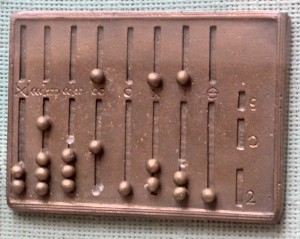
\includegraphics[scale=0.5]{RomanAbacusRecon.jpg}
\caption{로마시대 휴대용 주판 (복제품)\label{fig:RomanAbacus}\\
         \quad{\scriptsize (사진 출처: 위키미디어 공용)} }
\end{figure}

자연언어와 인공언어의 구분은 사람들끼리의 일상적인 의사소통을 위한 언어를
분류할 때 주로 사용하는 개념이다. 애초에 형식언어가 아닌 맥락에서 나온 개념이다.
형식언어도 인위적으로 만들었다는 점에서는 인공언어의 정의에도 부합하는 면이 있으나
그런 맥락에서는 사용하는 것은 일반적이지 않다. 그러니까 프로그래밍언어를
인공언어라고 해도 틀린 이야기는 아니지만 맥락에 따라 조금 어색한 표현일 수도 있다.
프로그래밍언어는 형식언어라고 이야기하는 것이 더 일반적인 표현이다.

컴퓨터 관련 분야에서 형식언어에 대비되는 개념, 즉 사람들끼리의 일상적인
의사소통을 위한 자연언어와 인공언어를 아우르는 용어는 그럼 무엇일까?
그냥 `자연언어'로 퉁친다. 왜냐하면 형식언어는 사람들끼리 일상적인
의사소통에 사용하는 언어들과는 워낙 그 특성이 동떨어져 있기 때문이다.
즉, 자연언어와 인공언어의 거리가 서울 부산 정도라면 형식언어는 달나라나
목성쯤에 있다고 비유할 수 있겠다. 인공지능 등의 기술로 한국어나 영어 등의
자연언어를 다루는 분야를 자연언어처리(natural language processing, NLP)라고 한다.
같은 기술로 에스페란토와 같은 인공언어를 처리한다 인공언어처리라고 부르지 않고
그냥 똑같이 자연언어처리로 취급할 따름이다.

\section{자연언어와 프로그래밍언에서 Syntax의 비중}
\label{sec:NatProgSyn}
언어학에서 음성 기반의 자연언어를 다룰 때는
작은 단위부터 큰 맥락까지 아래와 같이 다섯 같은 단계로 나눠 설명한다고 한다.
\begin{enumerate}\tightlist
    \item 음운론(phonology):
    소리의 단위인 음운을 다루는 이론.
    \item 형태론(morphology):
    의미의 단위인 형태소로 어휘를 구성하는 이론.
    \item 구문론(syntax):
    어휘로 문장을 구성하는 이론.
    \item 의미론(semantics):
    어휘나 문장이 갖는 의미에 대한 이론.
    \item 화용론(pragmatics):
    상황/문맥에 따른 어휘/문장의 활용을 다루는 이론.
\end{enumerate}
자연언어에서 문법(grammar)이란 음운론, 형태론, 구문론을 포괄하며 경우에 따라
의미론도 포함한다 \cite{IntroEngSem}. 자연언어 문장에서는 통사론적으로 같은
분류에 속하는 단어끼리도 원래의 단어를 다른 단어로 바꿔쳤을 때 그 의미의
차이에 따라 잘못된 문장으로 취급될 수도 있기 때문이다. 물론 자연언어에서도
구문론/통사론(syntax)이 문법(grammar)에서 다루는 핵심적인 부분이지만
그 외의 다른 요소들도 무시하지 못할 비중을 차지한다. 정리하면,
언어학에서 syntax는 grammar가 다루는 영역 중의 하나이므로
둘을 같은 우리말 용어로 옮겨 놓는다면 대단히 혼란스러울 것이다.

음성에 기반하지 않는 형식언어에서 음운론은 애초부터 논외이다.
프로그래밍언어 문법(syntax)의 대부분은 형식언어를 분류한 촘스키 계층
중에서 문맥자유언어(context-free language, CFL)에 해당한다.
문맥자유언어는 문법적으로 올바른 문장인지 판단하는 데 있어 의미나 맥락이
영향을 미치지 않으므로 형태론과 구문론만 고려하면 된다. 그런데 형식언어를
정의할 때에는, 예전부터 쓰던 어휘를 유지/계승해야 하는 자연언어와 달리, 
활용 목적에 알맞은 어휘를 새롭게 정하면 그만이므로 상대적으로 형태론의
비중도 미미하다. 따라서 프로그래밍언어에서 grammar는 syntax에 대한 내용을
주로 다루는 것이 당연하다. 즉, 프로그래밍언어에서는 syntax외에 grammar에서
다룰 내용이 거의 없으므로 둘 다 똑같이 `문법'으로 옮기더라도 그렇게 크게
혼란스럽지는 않을 것이다.

지금까지는 자연언어의 맥락에서 나온 용어들이 프로그래밍언어에서는 어떻게
그 번역이나 활용이 달라졌는지에 대해서 주로 이야기했다. 그런데 사실
형식언어에서 syntax와 grammar의 관계는 자연언어에서와는 조금 다른 관점에서
정리할 필요가 있다. 이에 대해서는 이어지는 절에서 좀더 이야기하기로 하자.

\section{형식언어이론에서 Syntax와 Grammar의 관계}
\label{sec:FormalLangSG}
형식언어이론(formal language theory, FLT)은 문장(정확히는 문자열)의 생김새(syntax)만을
대상으로 하며 그 뜻(semantics)은 생각하지 않는다. 형식언어이론에서 `언어'란 단순히
문자열(string)의 집합으로 정의된다. 문자열은 언어마다 미리 정해놓은 유한한 종류의
기호(symbol)를 한줄로 유한한 개수만큼 늘어놓아 만들어지며, 늘어놓은 기호의 개수가
바로 문자열의 길이가 된다. 형식언어에서 기호는 자연언어의 어휘(lexeme)에 대응되는 부분이다.
자연언어의 어휘는 의미의 최소단위인 형태소로 이루어지는 반면,
형식언어의 기호는 더 이상 쪼개지지 않고 의미가 부여되지 않는
원자적이고 추상적인 어휘에 해당한다.

이해를 돕기 위해 흑돌(\txtbullet)과 백돌(\txtcircle) 두 종류의 기호를 사용하는 형식언어
$L = \{\, \txtbullet\txtcircle
      ,\, \txtbullet\txtcircle\txtbullet\txtcircle
      ,\, \txtbullet\txtcircle\txtbullet\txtcircle\txtbullet\txtcircle
      ,\, \txtbullet\txtcircle\txtbullet\txtcircle\txtbullet\txtcircle\txtbullet\txtcircle
      ,\, \txtbullet\txtcircle\txtbullet\txtcircle\txtbullet\txtcircle\txtbullet\txtcircle\txtbullet\txtcircle
      ,\, \ldots
   \,\}$을 생각해 보라.
사실 기호의 표기상 그 모양이 바둑의 흑돌과 백돌처럼 보이기도 하기 때문에
편의상 그냥 `흑돌'과 `백돌'이라 부를 뿐이지 전혀 바둑과 관련된 의미를
부여하려는 것은 아니다. `꽉찬 동그라미'와 `빈 동그라미' 등으로 다르게
불러도 $L$의 정의는 젼혀 달라질 것이 없다. (더 나아가,
\txtbullet,\txtcircle 대신 $a$,$b$ 등으로 서로 구분되는
다른 어떤 두 기호라도 탐구하려는 형식언어의 본질이 달라지지는 않는다.)
이 언어에서 올바른 (즉, $L$의 원소인) 문자열의 특징을 설명하자면,\vspace{-1ex}
\begin{itemize}\tightlist
    \item[-] 가장 왼쪽 기호는 흑돌이고 가장 오른쪽 기호는 백돌이며
    \item[-] 같은 색 돌이 연속해 나타나지 않고 흑돌과 백돌이 번갈아 나타난다.
\end{itemize}
이와 같이 $L$에 속하는 문자열의 모양새가 어떠해야 하는지 제시하는 내용이
바로 언어 $L$ 의 syntax에 대한 표현이다. 이러한 내용은 언어 $L$의 고유한
성질을 알려줄 뿐이며 구체적으로 $L$에 속하는 문자열을 어떤 방법으로 어떤
과정을 거쳐 만들어내는지에 대해서까지 나타나 있지는 않다.

그렇다면 이번에는 좀더 구체적으로 문자열 \txtbullet\txtcircle\txtbullet\txtcircle를
만들어내는 방법을 생각해 보자. 굉장히 다양한 방법으로 만들어내는 것이 가능하며
그 중에서 다음의 몇 가지만 살펴보겠다.
\begin{enumerate}
    \item
    \fbox{\fbox{\fbox{\fbox{\!\txtbullet\!}\,\txtcircle\!}\,\txtbullet\!}\,\txtcircle\!}
    왼쪽 끝의 흑돌 하나로부터 오른쪽으로 하나씩 이어붙여서
    \item
    \fbox{\!\txtbullet\,\fbox{\!\txtcircle\,\fbox{\!\txtbullet\,\fbox{\!\txtcircle\!}}}}
    오른쪽 끝의 백돌 하나로부터 왼쪽으로 하나씩 이어붙여서
    \item
    \fbox{\fbox{\!\fbox{\!\txtbullet\!}\,\txtcircle\!}\,\fbox{\!\fbox{\!\txtbullet\!}\,\txtcircle\!}}
    흑돌 백돌 하나씩의 길이 2인 문자열이 두 번 반복되는 구조로
\end{enumerate}
$L$의 고유한 성질인 syntax를 표현하는 방식의 하나인 grammar를 어떻게 작성하느냐에
따라 만들어지는 결과물은 모두 \txtbullet\txtcircle\txtbullet\txtcircle로 같지만
그 문자열이 구성되는 방법과 만들어지는 과정이 달라질 수 있다. 즉, 같은 언어를 표현하는
서로 다른 grammar는 해당 언어에 속하는 문자열을 모두 만들어내므로 최종 결과물로 나오는
문자열들은 같지만, 만들어내는 구체적인 방식과 과정에는 차이가 있을 수 있다는 것이다.

지금까지 형식언어에서 syntax와 grammar가 어떤 식으로 관련된 개념인지 정리해 보았다.
형식언어의 계층적 분류 및 형식언어의 문법(grammar)에 대한 조금 더 자세한 이야기는
요점정리 후에 이어지는 다음 장에서 이어가기로 하자.

\section*{요점정리}
\begin{itemize}
    \item 프로그래밍언어란 좁은 의미에서는 기계(컴퓨터)에서 실행할 것을
    염두에 두고 만들어진 형식언어의 일종이지만 넓은 의미에서는 형식언어를
    모두 아우르는 개념이다.
    \item
    컴퓨터 분야에서 (형식언어 말고) `자연언어'라고 하면
    언어학에서 자연언어와 인공언어를 함께 아우르는 개념이다.
    \item
    프로그래밍언어 관련해서는 syntax와 grammar를 모두 `문법'이라고
    번역하는 경우가 많다. 둘은 관련된 개념이지만 구분할 필요가 있다.
    \item
    자연언어에서는 grammar가 다루는 여러 영역 중 하나가 syntax이다.
    \item
    형식언어의 syntax란 올바른 문자열의 모양새가 어떠해야 하는지 제시하는
    내용으로 특정 형식언어의 고유한 성질에 해당한다.
    \item
    형식언어의 grammar는 올바른 모양의 문자열을 만들어내기 위해
    사용하는 설계/시공 방법에 비유할 수 있다.
\end{itemize}


\chapter{형식언어이론}

형식언어이론에서는 어휘를 원자적 기호(symbol)로 추상화하여 의미를 부여하지 않으며,
기호의 나열로 이루어진 문자열(string)의 모양새(syntax)만을 기준으로 원하는 문자열을
골라 모아놓은 집합을 `언어'(language)로 규정한다. 문법(grammar)은 어떤 언어에 속하는
문자열을 만들어내는 과정을 안내하는 구체적인 규칙들로 이루어진다. 이런 문법을
어떤 식으로 정의하고 활용하는지 이 장에서 조금 더 자세히 소개한다. 그리고
문법(grammar)과 언어(language)의 모호성이 어떠한 개념인지 알아본다.
프로그래밍언어의 어휘(lexeme)와 구문(syntax)을 처리하는 데에도 형식언어이론을
활용하는데, 이런 활용에 있어서는 모호성을 피하는 것이 바람직하다.
프로그래밍언어에도 어휘분석(lexical analysis)보다 구문분석(syntax analysis)이
한층 더 복잡한 문제다. 따라서 어휘분석에 활용되는 형식언어보다 구문분석에 
활용되는 형식언어가 더 다루기 힘든 복잡한 성질을 가지고 있을 것이다.
형식언어의 복잡도에 따라 분류한 촘스키 계층 구조에 대해서도 소개한다.

이 책은 프로그래밍언어 분야에서 기본적으로 알아야 할 개념을 익히는
것을 목표로 하므로, 여기서는 형식언어이론을 체계적으로 다루기보다는
프로그래밍언어의 이해와 관련해 도움이 될만한 내용 위주로 간략하고 직관적으로 소개한다. 
형식언어이론에 전반에 대해 더 체계적으로 알아보려면 형식언어, 오토마타, 계산이론
등을 주제로 하는 교재\cite{Sipser2013,Hopcroft2007}를 참고하라.

\section{형식언어의 문법에 따른 문자열 생성}
\label{sec:GenGrammar}
형식언어의 문법(grammar)을 형식언어를 다룬다는 점을 강조하여 형식문법(formal grammar)이라
부르기도 한다. 형식언어이론에서 형식문법을 작성하는 표준적인 방식은 문자열을
만들어 나가는 과정을 안내하는 생성 규칙을 작성하며 이러한 방식로 문법을
표현한 것을 생성문법(generative grammar)이라고 한다. 형식언어의 문법
$G = \langle\, \Sigma, N, S, R \,\rangle$의 네 가지 요소는 다음과 같다.\vspace{-1ex}
\begin{itemize}\tightlist
    \item[$\Sigma$]: 생성된 문자열에 나타나는 단말 기호(terminal symbol)의 집합
    \item[$N$]: 생성 과정에 추가로 나타나는 비단말 기호(nonterminal symbol)의 집합
    \item[$S$]: 생성의 시작을 나타내는 시작 기호(start symbol) (단, $S\in N$)
    \item[$R$]: 생성 규칙(production rule)의 집합.
\end{itemize}

여기서 문법에 대해 구체적으로 소개하기 전에 형식언어란 문자열의 집합이며
문자열은 추상적인 어휘에 해당하는 `기호'로 이루어진다고 언급했는데,
그때 말한 기호가 바로 단말 기호에 해당한다.
그래서 단말 기호는 문법(grammar)과는 별개로 언어의 정의만으로도 결정된다.
앞서 \S\ref{sec:FormalLangSG}에서 예시로 들었던 흑돌과 백돌 기호를 사용한
언어에서 단말 기호의 집합 $\Sigma = \{\txtbullet, \txtcircle\}$이다.
최종 문자열을 생성하기 위한 추가적인 과정을 이어갈 필요가 없다는 뜻에서
`단말'이라는 표현을 쓴다고 이해해도 무방하다.

비단말 기호란 문자열의 생성 과정에서 단말 기호 이외에 추가로 나타나는
다른 기호를 말한다. 형식문법에서는 비단말 기호 중 하나를 시작 기호로
정해 놓아야 하므로 비단말 기호의 집합 $N$은 공집합일 수 없다. 시작 기호는
생성할 전제 문자열을 대표하는 기호로, 하나의 시작 기호($S$)로부터 문법의
생성 규칙에 따다 단계적으로 생성 과정을 거쳐 최종적으는 단말 기호만으로
이루어진 문자열이 만들어지게 된다. 생성 과정의 중간 단계에서는 비단말 기호만으로
이루어지거나 비단말과 단말 기호가 함께 나타나는 확장된 문자열의 개념이 필요하다.
문자열을 구성하는 바탕이 되는 기호의 집합을 알파벳(alphabet)이라 부른다.
최종 문자열의 알파벳은 단말 기호 집합($\Sigma$)이며 확장된 문자열의 알파벳은
단말과 비단말 기호의 합집합($\Sigma\cup N$)이다. 참고로 알파벳이 $X$인
모든 문자열의 집합을 $X^{*}$라 표기한다. 이를테면
$x$가 단말 기호를 알파벳으로 삼는 문자열이고
$\alpha$가 단말과 비단말 모두를 알파벳으로 삼는 문자열이라는
설명 대신 $x\in\Sigma^{*}$이고 $\alpha\in(\Sigma\cup N)^{*}$라고 쓰면 된다.

문법에서 가장 핵심적인 내용은 $\alpha\to\beta$ 형태의 생성 규칙(production rule)이다.
여기서 $\alpha$와 $\beta$는  $\Sigma\cup N$을 알파벳으로 하는 확장된 문자열인데,
단, $\alpha$는 길이 0인 빈문자열($\varepsilon$으로 표기)이 아니어야 한다
(즉, $\lvert\alpha\rvert>0$ 혹은 $\alpha\neq\varepsilon$).
시작 기호 하나로 이루어진 확장된 문자열 $S$로부터 시작해, 매 단계마다
문자열의 일부분(혹은 전체)가 화살표 왼쪽($\alpha$)과 일치하는 생성 규칙을
하나를 $R$에서 찾아 화살표 오른쪽($\beta$)의 내용으로 치환해 나가는 과정을
반복한다. 여러 생성 규칙의 화살표 왼쪽이 일치하는 경우에는 어떤 것을 선택해도 된다.
치환 결과로 나온 문자열 $x$가 비단말 없이 단말 기호로만 이루졌다면
성공적으로 문자열을 유도(derviation)한 것이며
$S\xRightarrow[\,G]{} \cdots \xRightarrow[\,G]{} x$ (단, $x\in\Sigma^{*}$)와 같이 표현한다.
만일 화살표의 왼쪽이 일치하는 생성 규칙을 $R$에서 찾을 수 없다면
최종 문자열 유도에 실패한 상황으로 생성 과정을 더 이상 진행할 수 없게 된다.
이렇게 문법 $G$의 생성 규칙에 따라 생성 가능한 모든 최종 문자열의 집합을
$\mathcal{L}(G)$로 표기한다.

\begin{figure}\centering
\begin{subfigure}[b]{0.4\textwidth}
\begin{align*}
G_1 & = \langle\, \Sigma, N_1, S_1, R_1 \,\rangle ~ \text{where}
\\ & \Sigma = \{\txtbullet,\txtcircle\}
\\ & N_1 = \{S_1,A_1\}
\\ & R_1 = \left\{
             \begin{array}{l}
             S_1 \to \txtbullet\,A_1 \,,\\
             A_1 \to \txtcircle\,S_1 \,,\\
             A_1 \to \txtcircle 
            \end{array}
           \right\}
\\ ~
\end{align*}
\end{subfigure}
\hfill
\begin{subfigure}[b]{0.35\textwidth}
\begin{align*}S_1
~\xRightarrow[\,G_1\!]{}~ & \txtbullet A_1
\\
~\xRightarrow[\,G_1\!]{}~ & \txtbullet \txtcircle\, S_1
\\
~\xRightarrow[\,G_1\!]{}~ & \txtbullet \txtcircle \txtbullet A_1
\\
~\xRightarrow[\,G_1\!]{}~ & \txtbullet \txtcircle \txtbullet \txtcircle
\\ ~
\end{align*}
\end{subfigure}
\hfill
\begin{subfigure}[b]{0.2\textwidth}\small
\begin{forest}
for tree={fit=tight, l sep-=.7em, l-=.7em}
  [$S_1$ [\txtbullet]
         [$A_1$ [\txtcircle]
                [$S_1$ [\txtbullet]
                       [$A_1$ [\txtcircle]]
                ]
         ]
  ]
\end{forest}\\
\end{subfigure}
\\
\begin{subfigure}[b]{0.4\textwidth}
\begin{align*}
G_2 & = \langle\, \Sigma, N_2, S_2, R_2 \,\rangle ~ \text{where}
\\ & \Sigma = \{\txtbullet,\txtcircle\}
\\ & N_2 = \{S_2,A_2\}
\\ & R_2 = \left\{
             \begin{array}{l}
             S_2 \to A_2\,\txtcircle \,,\\
             A_2 \to S_2\,\txtbullet \,,\\
             A_2 \to      \txtbullet
            \end{array}
           \right\}
\end{align*}
\subcaption*{grammar}
\end{subfigure}
\hfill
\begin{subfigure}[b]{0.35\textwidth}
\begin{align*}S_2
~\xRightarrow[\,G_2\!]{}~ & ~~~\; A_2\,\txtcircle
\\
~\xRightarrow[\,G_2\!]{}~ & ~~ S_2 \txtbullet \txtcircle
\\
~\xRightarrow[\,G_2\!]{}~ & A_2 \txtcircle \txtbullet\, \txtcircle
\\
~\xRightarrow[\,G_2\!]{}~ & ~ \txtbullet \txtcircle \txtbullet \txtcircle
\end{align*}
\subcaption*{derivation}
\end{subfigure}
\hfill
\begin{subfigure}[b]{0.2\textwidth}\small
\begin{forest}
for tree={fit=tight, l sep-=.7em, l-=.7em}
  [$S_2$ [$A_2$ [$S_1$ [$A_2$ [\txtbullet]]
                       [\txtcircle]
                ]
                [\txtbullet]
         ]
         [\txtcircle]
  ]
\end{forest}
\subcaption*{syntax tree}
\end{subfigure}
\caption{같은 언어에 대한 서로 다른 문법 $G_1$, $G_2$에 따른
         문자열의 유도(derivation) 및
         그에 대응되는 문법나무(syntax tree)
         \label{fig:OneLangTwoGrammar}
         }
\end{figure}

실제로 보기를 들어 설명하면 더 확실히 이해하는 데 도움이 될 것이다.
앞서 언급한 흑돌과 백돌을 기호로 하는 언어 
$L = \{\, \txtbullet\txtcircle
      ,\, \txtbullet\txtcircle\txtbullet\txtcircle
      ,\, \txtbullet\txtcircle\txtbullet\txtcircle\txtbullet\txtcircle
      ,\, \txtbullet\txtcircle\txtbullet\txtcircle\txtbullet\txtcircle\txtbullet\txtcircle
      ,\, \ldots
   \,\}$을 다시 생각해 보자.
언어 $L$의 문법 $G$를 정의한다는 말은 $L = \mathcal{L}(G)$를 만족하는 문법 $G$를 찾는
것과 같다. 한 언어의 문법은 유일하지 않고 여러가지로 정의할 수 있다.
그림\;\ref{fig:OneLangTwoGrammar}에는 $L = \mathcal{L}(G_1) = \mathcal{L}(G_2)$인
언어 $L$의 서로 다른 두 문법 $G_1$과 $G_2$의 정의가 나타나 있다. (사실은
언어 $L$을 표현하는 문법을 얼마든지 더 많이 다양하게 정의할 수 있다.)
문자열을 유도(derivation)하는 생성 과정은 마치 수식의 결과를 유도하는
계산 과정과 비슷하다. 차이점은 수식 계산이 큰 식을 점점 작게 하나의 값으로
줄이는 방향으로 진행되는 반면, 문자열 생성은 하나의 시작 기호를 점점 길게
전개하여 최종 문자열이 만들어지는 방향으로 진행된다. 문자열을 유도(derivation)하는
생성 과정에서는 매 단계마다 중간 과정에 중복된 정보의 표시가 많다. 예를 들면
그림\;\ref{fig:OneLangTwoGrammar}의 $G_1$에 따른 유도 과정의 첫 단계에서
생성된 가장 왼쪽의 \textbullet가 이후 단계에서 반복적으로 표기된다.
순차적으로 작성된 유도(derivation) 과정 대신에 도식적인 문법나무(syntax tree)의
형태로 표현하면 중복된 기호의 표시가 줄어들어 한눈에 알아보기 좋다.

참고로 프로그래밍언어에서 다루는 문법나무는 두 종류가 있다.
지금까지 다룬 그림\;\ref{fig:OneLangTwoGrammar}에 나타난 종류의 문법나무를
유도나무(derivation tree), 파스트리(parse tree), 또는
구체적 문법나무(concrete syntax tree) 등으로 부른다.
이와 상대되는 또다른 종류의 문법나무는
추상/요약 문법나무(abstract syntax tree)인데
이에 대해서는 다음 장(\S\ref{sec:LexParse})에서 다루기로 한다.

\section{문법과 언어의 모호성}
\label{sec:ambiguous}
앞절에서 예시로 살펴본 형식언어의 문법은 문맥자유문법(context-free grammar, CFG)이며
문맥자유문법으로 표현할 수 있는 형식언어를 문맥자유언어(context-free language, CFL)로
분류한다. 이 절에서는 문맥자유문법과 문맥자유언어의 `모호성'이라는 개념에 대해 알아본다.
문맥자유문법이나 문맥자유언어가 무엇인지는 다음 절에서 소개할 것이므로
지금은 `문맥자유'는 생략하고 그냥 (문맥자유)문법과 (문맥자유)언어라고 이야기하겠다.

하나의 문자열에 대해 서로 다른 여러 가지 문법나무를 구성할 수 있으면
모호한 문법이다. 앞서 그림\;\ref{fig:OneLangTwoGrammar}에서 살펴본
문법 $G_1$과 $G_2$는 모호하지 않다. 문자열을 한쪽 끝에서부터 한 글자씩
늘려 가며 다른 쪽 끝까지 생성하는 과정은 유일하므로 문법나무도 하나로
결정될 수밖에 없다. 그런데 같은 언어를 표현하는 또다른 문법 $G'$를
그림\;\ref{fig:ambG}에서와 같이 정의해 보자.
\begin{figure}\centering
\begin{subfigure}{0.45\linewidth}
\begin{align*}
G' & = \langle\, \Sigma, N', S', R' \,\rangle ~ \text{where}
\\ & \Sigma = \{\txtbullet,\txtcircle\}
\\ & N' = \{S'\}\cup N_1 \cup N_2
\\ & R' = \left\{\!\!
             \begin{array}{l}
             S' \to S_1 \,,\\
             S' \to S_2
            \end{array}
          \!\!\right\} \cup R_1 \cup R_2
\end{align*}
\end{subfigure}
\hfill
\begin{subfigure}{0.4\linewidth}\!\!\!\!\!\!\!\!
\begin{forest}
for tree={fit=tight, l sep-=.8em, l-=.8em}
[$S'$
  [$S_1$ [\txtbullet]
         [$A_1$ [\txtcircle]
                [$S_1$ [\txtbullet]
                       [$A_1$ [\txtcircle]]
                ]
         ]
  ]
] 
\end{forest}
~\quad~
\begin{forest}
for tree={fit=tight, l sep-=.8em, l-=.8em}
[$S'$
  [$S_2$ [$A_2$ [$S_1$ [$A_2$ [\txtbullet]]
                       [\txtcircle]
                ]
                [\txtbullet]
         ]
         [\txtcircle]
  ]
] 
\end{forest}
\end{subfigure}
\caption{모호한 문법 $G'$에 따른 같은 문자열에 대한 두 문법나무
         \label{fig:ambG}}
\end{figure}
문법 $G'$의 생성 규칙은 $G_1$과 $G_2$의 생성 규칙을 모두 포함하며
추가로 $G'$의 시작 기호에서 $G_1$의 시작 기호로 가는 규칙
($S'\to S_1$)과 $G_2$의 시작 기호로 가는 ($S'\to S_2$)으로
구성된다. 즉, $G'$에 따라 문자열 생성을 시작하면 $G_1$처럼 하든지
$G_2$처럼 하든지 둘 다 가능하다는 말이다. 그래서 문법 $G'$에
따라 \txtbullet\txtcircle\txtbullet\txtcircle를 생성하는 문법나무는
아래와 같이 두 가지가 가능하다. 따라서 $G'$는 모호한 문법이다.


지금까지 언어
$L = \{\, \txtbullet\txtcircle
      ,\, \txtbullet\txtcircle\txtbullet\txtcircle
      ,\, \txtbullet\txtcircle\txtbullet\txtcircle\txtbullet\txtcircle
      ,\, \txtbullet\txtcircle\txtbullet\txtcircle\txtbullet\txtcircle\txtbullet\txtcircle
      ,\, \ldots
   \,\}$의 문법 세 가지를 다뤘다. 그 중 둘($G_1$, $G_2$)은 모호하지 않았고
하나($G'$)는 모호했다. 그렇다면 이 언어는 태생적으로(inherently) 모호하지는 않다.
문법을 신경써서 잘 정의하면 모호하지 않은 문법으로 언어 $L$을 표현할 수 있기 때문이다.
한편, 언어 자체가 태생적으로 모호해서 아무리 노력해도 모호하지 않은 문법을
작성할 수 없는, 즉 어떤 언어 $L$에 대해 $L = \mathcal{L}(G)$를 만족하는
모호하지 않은 문법 $G$가 존재하지 않는 경우도 있다. 그런 언어는
(태생적으로, inherently) 모호하다고 말한다. 다음은 잘 알려진 모호한
(문맥자유)언어의 사례이다.
\[L_a = \{a^ib^jc^k \mid i=j ~\text{또는}~ j=k ~\text{($i,j,k$는 양의 정수) }\}\]
참고로 $a^i$는 기호 $a$가 $i$번 반복되 나열된 문자열을 말한다.
예컨대, $a^3 = aaa$이며 $a^3b^2c^2 = aaabbcc\,$이다.
위 언어의 모호성을 엄밀히 증명하려면 $L_a$를 표현하는 모든 가능한 문법을
다 시도해 보아도 불가능함을 보여야 하는데, 여기서는 그런 엄밀한 증명보다는
어떤 경우에 모호함을 해결하기 곤란한 상황인지만 짚고 넘어가기로 하겠다.
$L_a$의 문자열은 $a$와 $b$의 개수가 같거나 $b$와 $c$의 개수가 같거나 하는
둘 중 하나의 조건을 만족하면 된다. 각 조건을 만족하는 문자열에 대한
문법나무는 대략 아래와 같은 형태가 될 것이라 예상할 수 있다.
\begin{quote}
\begin{forest}
for tree={fit=tight, inner sep=0, l=0}
[$S$
 [$A_1$ [$a$,tier=word]
        [$A_1$ [$\cdots$,tier=word]
               [$\vdots$ [$a$,tier=word] [$b$,tier=word]]
               [$\cdots$,tier=word]
        ]
        [$b$,tier=word]]
 [$B_1$ [$c\cdots c$, roof, tier=word]]
]
\end{forest}
\qquad\qquad
\begin{forest}
for tree={fit=tight, inner sep=0, l=0}
[$S$
 [$A_2$ [$a\cdots a$, roof, tier=word]]
 [$B_2$ [b,tier=word]
        [$B_2$ [$\cdots$,tier=word]
               [$\vdots$ [b,tier=word] [c,tier=word]]
               [$\cdots$,tier=word]
        ]
        [c,tier=word]]
]
\end{forest}
\end{quote}
그런데 두 가지 조건을 동시에 만족하는 경우는 어떨까? 즉, $i=j=k$로 $a$, $b$, $c$ 세
기호의 개수가 모두 같은 $aaabbbccc$같은 경우 말이다. 이런 문자열의 경우에는
$a$와 $b$를 쌍쌍이 생성하며 개수를 맞추는 왼쪽의 형태로도
$b$와 $c$를 쌍쌍이 생성하며 개수를 맞추는 오른쪽의 형태로도
처리할 수 있다는 모호함이 있다. 이는 언어 $L_a$의 본질적인 성질이라
문법을 달리 정의하려 하더라도 비본질적인 변화만을 줄 뿐 하나의 문자열을
생성하는 문법나무가 여러 가지로 가능해지는 것을 피하지 못한다.


\section{촘스키 계층}
\begin{figure}\centering
\begin{subfigure}{.25\textwidth}
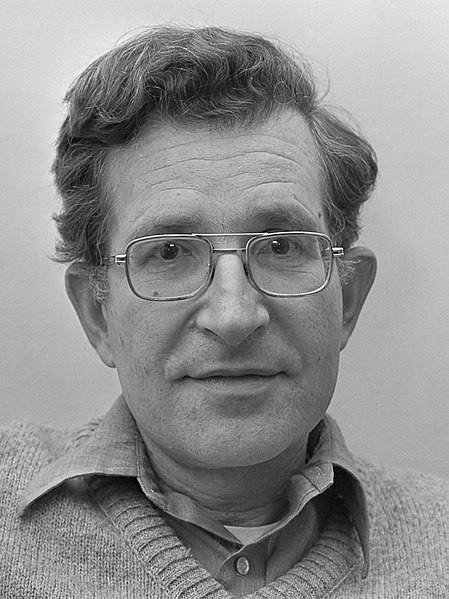
\includegraphics[]{Chomsky1977.jpg}
\end{subfigure}
\begin{subfigure}{.6\textwidth}
\begin{tabular}{lcrl}
Type-0\!\!\!\!\!\!&(무제약)  &\!\!\!\!\!\!문법:& $\alpha\to\gamma$
\\    \!\!\!\!\!\!&$^{\text{unrestricted}}$& \\
Type-1\!\!\!\!\!\!&(문맥의존)&\!\!\!\!\!\!문법:& $\alpha A\beta\to\alpha\gamma\beta$
\\    \!\!\!\!\!\!&$^{\text{context-sensitive}}$& \\
Type-2\!\!\!\!\!\!&(문맥자유)&\!\!\!\!\!\!문법:& $A\to \gamma$
\\    \!\!\!\!\!\!&$^{\text{context-free}}$& \\
Type-3\!\!\!\!\!\!&(정규)    &\!\!\!\!\!\!문법:& $A\to a$, $A\to bB$
\\    \!\!\!\!\!\!&$^{\text{regular}}$&
\end{tabular}
\begin{center}
\quad$a,b\in \Sigma$,\quad$A,B\in N$,\quad$\alpha,\beta,\gamma\in(\Sigma\cup N)^{*}$
\end{center}
\end{subfigure}
\caption{촘스키의 1977년 사진 및 촘스키 계층별 문법의 생성규칙 형태
         \label{fig:ChomskyHierarchyGrammar}\\
         {\scriptsize(사진 출처: 위키미디어 공용)} }
\end{figure}
\noindent
촘스키는 문법에서 생성규칙의 형태를 얼마나 제약하는가를 기준으로 형식문법을
네 계층으로 분류하였는데\cite{Chomsky56}, 이를 촘스키 계층(Chomsky hierarchy)이라고
한다 (그림\;\ref{fig:ChomskyHierarchyGrammar}).
촘스키 계층의 문법은 Type-0부터 Type-3까지의 번호가 들어간 이름으로도,
또 그 특성을 드러낸 이름으로도 불린다. 이를테면 ``Type-3 문법''과
``정규문법''(regular grammar)은 같은 뜻의 용어이다. 번호가 작을수록
제약이 적기 때문에 더 다양한 형태의 문법 규칙이 허용되며 번호가 클수록
더 제한된 형태의 문법 규칙만이 허용된다. 따라서 Type-0이 생성문법의
가능한 모든 규칙이 허용되는 가장 큰 문법의 범주이며, Type-1은 Type-0의 일부분,
Type-2는 Type-1의 일부분, Type-3은 Type-2의 일부분이다. 즉,
모든 정규문법은 문맥자유문법이기도 하고, 모든 문맥자유문법은 문맥의존문법이기도 하며,
모든 문맥의존문법은 무제약문법이기도 하다.

무제약 문법(unrestricted grammar)은 생성규칙의 형태에 아무런 제약 없이
화살표의 왼쪽과 오른쪽에 아무런 확장된 문자열이나 다 쓸 수 있다. 예를 들면
$bABa \to aBbaAb$같은 복잡한 규칙도 허용된다. 그러니까 문자열의 생성 과정에서
임의 개수의 단말과 비단말을 또다른 임의 개수의 단말과 비단말로 바꿔나갈 수 있다.
무제약 문법으로 표현가능한 언어의 범주를
`재귀열거언어'(recursively enumerable language)라 한다.

문맥의존문법(context-sensitive grammar, CSG)은 화살표 왼쪽에서 비단말 기호 하나만을
치환하며 생성해 나가는 규칙만 허용한다. $\alpha A\beta\to\alpha\gamma\beta$ 형태의
규칙은 $\alpha$와 $\beta$ 사이에 나타나는 비단말 기호 $A$를 $\gamma$로 치환하라는 뜻이다.
이 규칙으로는 $A$의 앞과 뒤에 $\alpha$와 $\beta$가 나타나지 않으면
$A$를 $\gamma$로 치환할 수 없다. 문맥의존문법으로 표현가능한 언어의 범주를
`문맥의존언어'(context-sensitive language, CSL)라 한다.

문맥자유문법(context-free grammar, CFG)은 문맥의존문법의 생성규칙 형태인
$\alpha A\beta\to\alpha\gamma\beta$에서 $\alpha$와 $\beta$ 모두 길이 0인
빈 문자열이라는 (즉, $\alpha=\beta=\varepsilon$) 추가적인 제약이 있는 셈이다.
즉, 문맥자유문법 생성규칙 $A\to\gamma$에 따르면 $A$의 주변에 무엇이 있든 없든
관계없이 $A$를 어디서나 $\gamma$로 치환할 수 있다. 문맥자유문법으로 표현가능한
언어의 범주를 `문맥자유언어'(context-free language, CFL)라 한다.

정규문법(regular grammar)은 문맥자유문법의 생성규칙 형태인 $A\to\gamma$에서
화살표 오른쪽 $\gamma$의 형태를 단말 기호 하나($a$) 또는
단말과 비단말 기호 하나씩($bB$)으로 추가적으로 제한한 것이다.
정규문법으로 표현가능한 언어의 범주는 `정규언어'(regular language)이다. 
참고로 정규언어는 생성규칙의 형태로 표기하기에는 너무 간단한 언어라서
정규문법 대신에 `정규식'(regular expression)으로 표현하여 활용하는 경우가 많다.
정규식에 대해서는 다음 장에서 프로그래밍언어의 어휘분석을 다루면서 설명하겠다.

\begin{figure}[b]\centering
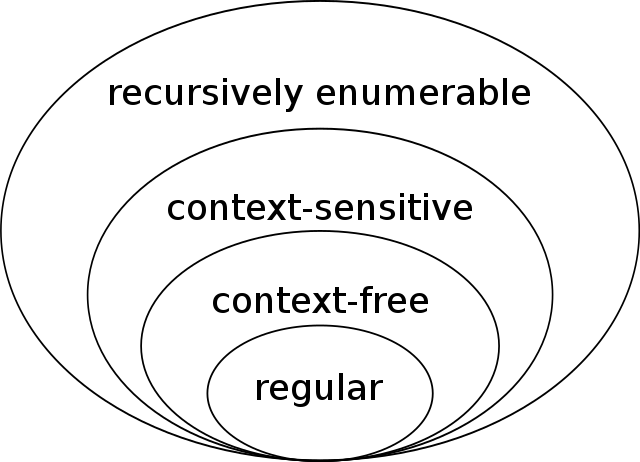
\includegraphics[scale=0.5]{ChomskyHierarchy.png}
\caption{촘스키 계층의 문법에 대응되는 언어 범주의 포함관계
         \label{fig:ChomskyHierarchyLang}\\
         {\scriptsize(이미지 출처: 위키미디어 공용)} }
\end{figure}

정규언어는 여러 번 반복되는 구조가 나타나는 포함할 수 있지만
문자열의 특정 지점까지 몇 번이나 반복했는지 그 회수를 기억해
이후의 문자이 어떤 내용이 되어야 언어에 포함시킬지에 판별하는 데
영향을 미칠 수 없다는 것이 특징적인 성질이다. 예제로 다루던 언어
$L = \{\, \txtbullet\txtcircle
      ,\, \txtbullet\txtcircle\txtbullet\txtcircle
      ,\, \txtbullet\txtcircle\txtbullet\txtcircle\txtbullet\txtcircle
      ,\, \ldots
   \,\}$는 $\txtbullet\txtcircle$이 1회 이상 반복되어 나타나는
모든 문자열로 이루어져 있는 정규언어이다.
하지만 언어 $L_p = \{\txtbullet^n\txtcircle^n \mid n>0\}$는
정규언어가 아니다. 왜냐하면 백돌이 나타나기 전까지 흑돌의 개수를
기억했다 후반부에 나타나는 백돌의 개수와 맞춰봐야 $L_p$에 포함되는
문자열인지 구분할 수 있기 때문이다. 그래서 정규언어로는 괄호의 쌍을
맞추도록 처리하는 것이 불가능하다. 괄호가 이전까지 몇 번 열렸는지
기억하고 있어야 그에 쌍을 맞춰 괄호를 닫을 수 있는데 정규언어는
그보다 더 단순히 회수를 기억하지 못하는 반복 구조만을 다룰 수 있다.

정규언어의 범주를 넘어선 문백자유언어의 범주에서는 괄호를 맞출 수 있다.
문맥자유문법 $G_p =
   \left\langle\, \{\txtbullet,\txtcircle\},\, \{S,A\},\, S,\,
                  \{\,S\to\txtbullet\,\txtcircle,\,S\to\txtbullet\,S\,\txtcircle\,\}
\,\right\rangle$로 바로 위에서 정규언어가 아닌 예로 들었던 언어 $L_p$를 표현할 수 있다.
$L_p$의 문자열인 \txtbullet\txtbullet\txtcircle\txtcircle를 $G_p$에 따라
다음과 같이 생성할 수 있다.
\begin{center}
\begin{forest}
for tree={fit=tight, l sep-=.5em, inner sep=0, l=0}
[$S$ [\txtbullet,tier=word]
     [$S$ [\txtbullet,tier=word] [\txtcircle,tier=word]]
     [\txtcircle,tier=word]
]
\end{forest}
\end{center}
이렇듯 문맥자유언어의 범주에서는 쌍을 맞춰가며 개수를 비교해 언어에 포함되는
문자열인지 판단할 수 있다. 그러나 그보다 더 복잡한 구조에서 개수를 비교해
문자열이 언어 포함되는지 따지는 것은 불가능하다. 서로 다른 세 문자가 모두
같은 개수만큼 차례로 나타나는 $\{a^nb^nc^n\mid n>0\}$은 문맥자유언어가 아닌 예로
잘 알려진 언어이다. 나란히 있는 $a$와 $b$끼리 또는 $b$와 $c$끼리 쌍을 맞춰가거나
아니면 가운데 $b$를 남겨놓고 $a$와 $c$끼리 쌍을 맞춰가며 개수를 비교할 수는 있지만,
동시에 세 부분의 개수를 맞는지 따지는 것은 문맥자유언어의 범주에서 불가능하다.
참고로 $\{a^nb^nc^n\mid n>0\}$는 문맥의존문법으로 표현가능한 문맥의존언어의 범주에 속한다.


\section*{요점정리}
\begin{itemize}
    \item 형식언어이론에서 언어란 문자열의 집합으로 정의된다.
    \item 형식언어의 문법 $G=\langle\Sigma,N,S,R\rangle$은
    최종 문자열을 구성하는 단말 기호의 집합($\Sigma$),
    생성 도중에만 나타나는 비단말 기호의 집합($N$),
    생성 과정의 처음을 나타내는 시작 기호($S$),
    생성 규칙의 집합($R$)의 네 요소로 정의된다.
    \item 문법의 핵심적인 요소인 $\alpha\to\beta$의 형태의 생성 규칙에 따라
    화살표 왼쪽에 나타나는 확장된 문자열($\alpha$)을 오른쪽에 나타나는
    확장된 문자열($\beta$)로 치환해 나가는 과정을 단말 기호로만 이루어진
    문자열이 생성되기까지 반복한다.
    \item 문법 $G$가 언어 $L$을 표현한다는 것은 문법에 따라 생성 가능한 모든
    문자열의 집합이 주어진 언어와 일치, 즉 $\mathcal{L}(G) = L$임을 뜻한다.
    일반적으로 하나의 언어를 표현하는 문법은 여러가지로 작성 가능하다.
    \item 문자열 유도(derivation) 과정의 순차적 나열 대신
    문법나무(syntax tree)의 형태로 표현하면 중복된 표기가 줄어들어
    한눈에 알아보기 좋다.
    \item 같은 문자열을 생성하는 서로 다른 문법나무가 여럿인 경우가
    있다면 모호한 문법이다.
    \item 언어를 표현하는 문법이 모두 모호한 경우, 즉 아무리 신경써서
    문법을 작성해도 모호하지 않은 문법으로는 표현할 수 없는 경우에
    (태생적으로) 모호한 언어라고 한다.
    \item 촘스키는 생성규칙 형태의 제약 정도에 따라 문법을 네 계층으로 분류하였으며
    (정규$\,\subset\,$문맥자유$\,\subset\,$문맥의존$\,\subset\,$무제약),
    그에 대응되는 언어의 범주도 네 계층을 이룬다
    (정규$\,\subset\,$문맥자유$\,\subset\,$문맥의존$\,\subset\,$재귀열거).
    \item 정규언어의 범주에서는 회수를 기억하지 않는 한에서 반복된 구조를
    판별할 수 있으며, 문맥자유언어의 범주에서는 여닫는 괄호의 개수를 맞추는
    것과 같이 쌍을 맞춰가는 반복된 구조를 판별할 수 있다.
\end{itemize}

\section*{연습문제}
\begin{enumerate}
\item 다음 문맥자유언어에 대한 형식문법을 작성해 보라.\\
$\displaystyle
 \left\{ \mathtt{d}\mathtt{s}^n\mathtt{o}\mathtt{z}^n\mathtt{b}
           \mid
           n\ge0 \right\}
 =
 \left\{ \mathtt{dob}
       , \mathtt{dsozb}
       , \mathtt{dssozzb}
       , \mathtt{dsssozzzb}
       , \ldots \right\}$

\item 다음 문맥자유언어에 대한 형식문법을 작성해 보라.\\
$\displaystyle
 \left\{ \mathtt{w}^n\mathtt{o}\mathtt{v}^{2n}
           \mid
           n\ge1 \right\}
 =
 \left\{ \mathtt{wov}
       , \mathtt{wwovvvv}
       , \mathtt{wwwovvvvvv}
       , \ldots \right\}$
\end{enumerate}

\chapter[프로그래밍언어의 문법구조(Syntax)]{프로그래밍언어의\\문법구조(Syntax)}
프로그래밍언어의 설명서는 어휘구조(lexical structure)라는 항목이
등장하며, 어휘가 모여 어떻게 구문구조(syntax)를 이루는지에 대한
설명도 이어진다. 그렇게 `-구조'를 붙여 우리말로 옮기는 것과 일관되게
프로그래밍언어의 겉모양과 속뜻에 해당하는 용어를 문법구조(syntax)와
의미구조(semantics)로 옮기기도 한다. 이 장에서는 프로그래밍언어의
문법구조와 관련된 개념과 용어를 소개한다.

어휘구조(lexical structure)와 나란히 쓰이는 구문구조(syntax)와
의미구조(semantics)와 나란히 쓰이는 문법구조(syntax)의
syntax는 같은 영어 단어라도 다른 맥락에서 쓰이는 조금 다른 개념이다.
두 개념을 함께 다룰 때는 그 차이가 분명히 드러나도록
전자를 ``구체적 문법''(concrete syntax) 후자를
``추상(또는 요약) 문법''이라고 구분하여 부르기도 한다.
이 장에서 설명할 내용을 통해 이렇게 비슷하지만 다른 맥락에서
조금씩 다른 개념으로 쓰이는 용어를 구별하여 이해하는 데 도움이
되기를 바란다.

\newpage

\section{어휘 및 구문 분석}
\label{sec:LexParse}
프로그래밍언어의 설명서\cite{Swift5Ref,CSharp6Draft,JavaSE8spec,Haskell2010}에서
흔히 어휘구조(lexical structure)라는 항목 하에 글자들이 모여 어떤 종류의
어휘를 이루는지, 그러니까 리터럴(literal), 식별자(identifier), 연산자(operator),
키워드/예약어(keyword/reserved word), 주석(comment) 등이 되는지 설명한다.
그런 어휘가 모여 어떻게 구문구조(syntax)를 이루는지를 다루는 내용은
어휘구조에 비해 더 복잡하므로 식(expression), 문(statement), 블럭(block) 등의
요소별로 별도의 항목으로 나누어 설명하는 것이 일반적이다.

프로그래밍언어의 소스코드는 일차원적으로 나열된 문자열로 작성되어 있다.
이렇게 한줄로 이어진 문자열로부터 어휘분석(lexical analysis) 단계를 거치면
하나 혹은 그 이상의 글자들로 이루어진 어휘(lexeme)를 각각 끊어냄으로써
어휘구조를 인식하고, 각각 어떤 종류의 어휘인지 구별된 토큰(token)의
나열인 토큰열을 얻는다. 토큰열로부터 문법분석(syntax analysis) 단계를
거치면 구문구조를 인식하며 구체적문법나무(concrete syntax tree)를 구성하고,
그 핵심만을 요약한 추상문법나무(abstract syntax tree, AST)를 얻는다.
그림\;\ref{fig:LexParse}에는 뺄셈, 곱셈, 거듭제곱 연산을 포함한
산술식(arithmetic expression)을 예시로 어휘분석 및 구문분석 과정에서
나타나는 네 가지 데이터 구조들인 문자열, 토큰열, 구체적문법나무,
추상문법나무가 한눈에 잘 알아볼 수 있도록 나타나 있다.
그림\;\ref{fig:LexParse}의 각 구조에 대해 예시를 중심으로 조금
더 알아보자.

\begin{figure}\centering
\setlength{\tabcolsep}{.8ex}
\renewcommand{\arraystretch}{1}
\begin{subfigure}{.8\textwidth}\ttfamily
\begin{tabular}{| *{25}{m{.8ex}|} }
\hline 
5& &*& &(& & & &1&0& &-& &8&)& &*& &2&\char`^&2& &\char`^& &3\\
\hline
\end{tabular}
\caption{문자열(sequence of characters)\label{sfig:charseq}}
\end{subfigure}
~\\
\hfill
\begin{subfigure}{.6\textwidth}\ttfamily
~\\[1ex]
\fbox{$5$}
\fcolorbox{teal}{teal!20}{*}
\fcolorbox{brown}{brown!20}{(}
\fbox{$10$} \fcolorbox{teal}{teal!20}{-} \fbox{$8$}
\fcolorbox{brown}{brown!20}{)}
\fcolorbox{teal}{teal!20}{*}
\fbox{$2$}
\fcolorbox{teal}{teal!20}{\textbf{\char`^}} \fbox{$2$}
\fcolorbox{teal}{teal!20}{\textbf{\char`^}} \fbox{$3$}
\caption{토큰열(sequence of tokens)\label{sfig:tokseq}}
\end{subfigure}
\\[-7ex]
\qquad
\begin{subfigure}[b]{.4\textwidth}
\begin{forest}
for tree={l sep-=.8em, l-=.8em, inner sep=0, l=0}
[$E$ [$T$, for current={s sep=+2em}, for children={s sep+=1em}
  [$T$ 
       [$F$ [$A$ [$5$]]]
       [$*$]
       [$F$ [$A$, for current={s sep+=1em}
         [$($]
         [$E$
           [$E$ [$T$ [$F$ [$A$ [$10$]]]]]
           [$-$]
           [$T$ [$F$ [$A$ [$8$]]]]
         ]
         [$)$]
       ]]
  ]
  [$\phantom{a}\quad*\quad\phantom{a}$]
  [$F$
    [$A$ [$2$]]
    [\textbf{\char`^}]
    [$F$ [$F$ [$A$ [$2$]]] [\textbf{\char`^}] [$A$ [$3$]]]
  ]
]]
\end{forest}
\subcaption{구체적문법나무\\(concrete syntax tree)\label{sfig:CST}}
\end{subfigure}
\hfill
\begin{subfigure}[b]{.4\textwidth}\centering\ttfamily
\begin{forest}
for tree={inner sep=0, l sep+=1em, l=0}
[*,circle,draw,for current={s sep+=1em}
   [*,circle,draw,for current={s sep+=1em}
      [$5$]
      [-,circle,draw [$10$] [$8$]]
   ]
   [\textbf{\char`^},circle,draw,for current={s sep+=1em}
      [$2$]
      [\textbf{\char`^},circle,draw [$2$] [$3$]]
   ]
]
\end{forest}
\subcaption{추상문법나무(요약문법나무)\\(abstract syntax tree)\label{sfig:AST}}
\end{subfigure}
\caption{\lstinline[columns=flexible
                   ,keepspaces=true
                   ,showspaces=true]|"5 * ( {} {} 10 - 8) * 2^2 ^ 3"|에 대한
         어휘분석 과정({\scriptsize(a)$\to$(b)})과 
         구문분석 과정({\scriptsize(b)$\to$(c)$\to$(d)})에 나타나는 데이터 구조들
         \label{fig:LexParse}}
\end{figure}

그림\;\ref{sfig:charseq}는 문자열
\lstinline[columns=flexible
                   ,keepspaces=true
                   ,showspaces=true]|"5 * (   10 - 8) * 2^2 ^ 3"|를
이루는 각각의 글자(character)를 일차원적인 공간에 차례대로 배치하고 있다.
(참고로, 여기서는 공백 문자임을 강조하기 위해 빈칸으로 나타내는 대신
\lstinline[columns=flexible
                   ,keepspaces=true
                   ,showspaces=true]| |로 표시하였다.)
이 문자열은 0부터 9까지 십진수 숫자(digit); 뺄셈, 곱셈, 거듭제곱 등의
산술 연산을 나타내는 기호; 열고 닫는 괄호 기호; 그리고 공백 문자로
이루어져 있다. 들여쓰기로 블럭을 구분하거나 공백 없이 붙여쓰면 하나의
어휘로 인식되는 경우를 제외하면, 사람의 눈에 알아보기 좋은 소스코드가
되도록 공백 문자를 적당히 추가하더라도 내용에는 실제적인 영향을
미치지 못하는 경우가 대부분이다. 즉,
\lstinline[columns=flexible
                   ,keepspaces=true
                   ,showspaces=true]|"5*(10-8)*2^2^3"|처럼
공백을 제외한 문자열도 똑같은 수식을 표현하게 된다.

그림\;\ref{sfig:tokseq}는 앞서 언급한 문자열의 어휘분석 결과로 나온
토큰열을 나타낸다. 5나 \texttt{*}와 같이 하나의 글자로 된 어휘도 있지만
10과 같이 두 개 이상의 글자가 모여 하나의 어휘를 이루기도 한다.
문자열에서 어휘를 끊어내면서 어휘 사이의 공백 문자는 버린다.
단지 어휘를 끊어낼 뿐만 아니라 어휘의 종류를 구분하여 정리해 놓는데,
이렇게 종류가 구분된 어휘를 토큰(token)이라고 한다.
5, 10, 6 등은 정수 리터럴(integer literal),
\texttt{*}, \texttt{-}, \texttt{\textbf{\char`^}} 등은 연산자,
열고 닫는 괄호 등의 토큰으로 구분됨을 색상으로 표시하였다.
결과로 토큰열을 얻으므로 어휘분석을 토큰화(tokenization)라고도 한다.
프로그래밍언어 분야에서는 어휘분석(lexical analysis)을 줄여
렉싱(lexing)이라 부르는 경우가 많다. 따라서 어휘분석을 수행하는
프로그램인 어휘분석기(lexical analyzer)를 토크나이저(tokenizer)라고도 하며,
프로그래밍언어의 경우 렉서(lexer)라 부르는 경우가 많다.

구문분석(syntax analysis)은 언어학 및 컴퓨터 관련 분야에서
파싱(parsing)이라고도 한다. 참고로 파싱(parsing)의 어원이 되는 동사
parse는 품사(parts of speech)를 뜻하는 라틴어에서 유래했다\cite{MWdict}.
즉, parse란 문장을 구성하는 각 부분이 문법적으로 어떤 부류에
속하는지 인식해 문장의 구조를 분석한다는 뜻으로 이해할 수 있다.
구문분석을 수행하는 프로그램인 구문분석기(syntax analyzer)를
컴퓨터 관련 분야에서 파서(parser)라 부르는 경우가 많다.
프로그래밍언어의 파서는 토큰열(그림\;\ref{sfig:tokseq})로부터
구체적문법나무(그림\;\ref{sfig:CST})를 구성하고 이를 요약한
추상문법나무(그림\;\ref{sfig:AST})를 만들어낸다. `추상문법나무'는
프로그래밍언어의 의미를 다루기 위한 핵심적 부분만을 요약하고 있으므로
`요약문법나무'로도 옮긴다. 또한 구체적문법나무(concrete syntax tree)와
요약문법나무(abstract syntax tree)대신 파스나무(parse tree)와
문법나무(syntax tree)로도 일컫는다. 파서(parser)의 최종 결과물은
파스나무(즉, 구체적문법나무)가 아니라 문법나무(즉, 요약문법나무)다.

정리하면, 프로그래밍언어의 문법(syntax)을 두 단계로 구분해 생각할 수 있다.
첫째는 토큰열로부터 구체적문법나무를 구성하기 위한
구체적문법(concrete syntax), 둘째는 요약문법나무의 구조를
나타내는 요약문법(abstract syntax)이다. 물론 요약문법을
추상문법이라고도 옮긴다. 용어의 다양한 우리말 옮김에 대해서는
충분히 소개했으니 이제부터 이 책에서는 `추상-'보다는 `요약-'이 붙은
용어를 사용하기로 한다. 이어지는 절(\S\ref{sec:GrammarNotation})에서는
구체적문법과 요약문법의 표기방법에 대해 대해 먼저 알아보고,
그 다음 절(\S\ref{sec:regex})에서 어휘분석에 활용되는 정규식에
대해 알아보기로 하자.

\section{문법의 표기}
\label{sec:GrammarNotation}
앞절에서 정리한 바와 같이, 프로그래밍언어의 구체적문법은 일차원적 구조인
토큰열로부터 구체적문법나무를 하나로 결정할 수 있어야 하므로 모호함 없는
(unambiguous) 문맥자유문법으로 정의되어야 한다. 참고로 문맥자유문법에서
모호함의 개념에 대해서는 \S\ref{sec:ambiguous}에서 다룬 바 있다.
프로그래밍언어의 문법에서 모호함을 해소해야 하는 대표적인 요소로
연산자(operator)의 우선순위(precedence)와 결합성(associativity)을 들 수 있다.
우선순위는 서로 다른 연산자들 사이에 어느 연산자가 우선하는지를 말한다.
보통 곱셈과 나눗셈 연산이 덧셈과 뺄셈 연산보다 우선순위가 높으므로
$8\mathop{\texttt{-}} 3\mathop{\texttt{*}}2 $는
$8\mathop{\texttt{-}}(3\mathop{\texttt{*}}2)$와 같은 의미다.
결합성은 같은 연산자가 연달아 사용하는 것이 가능한지 그리고
가능하다면 어떤 방향으로 결합이 우선하는지를 말한다.
보통 좌결합(left-associative)인 뺄셈의 경우
$ 8\mathop{\texttt{-}}3 \mathop{\texttt{-}}2$는
$(8\mathop{\texttt{-}}3)\mathop{\texttt{-}}2$와 같고
우결합(right-associative)인 거듭제곱의 경우
$2\mathop{\texttt{\char`^}} 2\mathop{\texttt{\char`^}}3 $는
$2\mathop{\texttt{\char`^}}(2\mathop{\texttt{\char`^}}3)$와 같은 의미다.
그리고 기본적인 연산자 우선순위 및 결합성과 달리 순서를 명시적으로
강제하기 위한 괄호(parenthesis) 또한 구체적문법에 포함되곤 한다.
요약문법은 이미 구체적문법으로 모호함 없이 분석된 바를 요약한 구조만을
다루므로 일차원적 구조의 처리와 관련된 모호성을 신경쓸 필요가 없다.
따라서 요약문법에는 연산자 우선순위나 결합성을 고려할 필요가 없으며
괄호와 같이 우선순위를 명시적으로 강제하는 요소도 나타나지 않는다.
이제 사칙연산(\texttt{+}, \texttt{-}, \texttt{*}, \texttt{/})과
거듭제곱(\texttt{\char`^})을 포함한 산술식에 대한 구체적문법과
요약문법의 표기에 대해 알아보자.

그림\;\ref{fig:BNF}는 똑같은 산술식의 구체적문법(concrete syntax)을
나타내는 형식문법의 생성규칙과 BNF 표현을 나란히 비교하고 있다.
참고로 화살표 왼쪽이 같은 비단말인 생성규칙끼리 묶어 간략하게 표기하기도 한다.
예를 들면 세 개의 규칙
$E \to E ~\texttt{+}~ T$, $E \to E ~\texttt{-}~ T$, $E \to T$를
한꺼번에 $E \to E\;\texttt{+}\;T \mid E\;\texttt{-}\;T \mid T$로
묶어 표기한다. 그림\;\ref{fig:BNF}의 생성규칙도 이렇게 묶어 표기한 형태로
그 바로 옆에 나란히 나타난 BNF 표현의 구조와 일치한다.
즉, 비단말 $E$, $T$, $F$, $A$, $Z$를 각각 \texttt{<expr>},
\texttt{<term>}, \texttt{<factor>}, \texttt{<factor>},
\texttt{<atom>}, \texttt{<integer>}에 대응시키고, 단말은
쌍따옴표(\texttt{"})로 둘러싸고, $\to$를 \texttt{::=}로
바꾸기만 하면, 생성규칙을 BNF로 옮길 수 있다. 형식문법의 생성규칙은
마치 수학에서 수식과 같이 주로 이론적 논의를 위한 간결함을 우선시하여
비단말은 대문자 단말은 소문자 한 글자씩만으로 표시한다.
프로그래밍언어 분야에 선구적 업적을 남긴
두 컴퓨터 과학자(그림\;\ref{fig:BackusNaur})의 이름을 딴
배커스--나우르 형식(Backus--Naur Form, BNF)은 프로그래밍언어의
구체적문법을 정의하는 등의 실용적인 활용을 염두에 두고 만들어졌다.
BNF는 알아보기 쉬운 단어로 비단말을 표현하거나 여러 글자로 된 단말의
표현도 가능한, 실용적 편의성을 고려된 문맥자유문법의 표기 방식이다.

\begin{figure}\centering
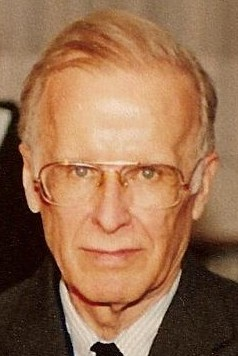
\includegraphics[scale=0.25]{JohnBackus.jpg}
\qquad\qquad\qquad
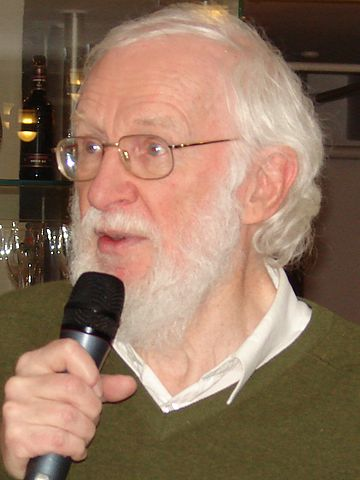
\includegraphics[scale=0.21]{PeterNaur.jpg}
\caption{Fortran 언어의 창시자인 John Backus(1999년 사진, 좌)와\\
         ALGOL 60 언어 개발을 주도한 Peter Naur(2008년 사진, 우)\\
         {\scriptsize(사진 출처: 위키미디어 공용)}\label{fig:BackusNaur}}
\end{figure}
\begin{figure}[H]\vspace*{-4ex}
\hfill
\begin{subfigure}[b]{.2\linewidth}\addtolength{\jot}{-.3em}
\begin{align*}
E \to~& E ~\texttt{+}~ T \\
 \mid~& E ~\texttt{-}~ T \\
 \mid~& T \\
T \to~& T ~\texttt{*}~ F \\
 \mid~& T ~\texttt{/}~ F \\
 \mid~& F \\
F \to~& A ~\texttt{\char`^}~ F \\
 \mid~& A \\
A \to~& Z \\
 \mid~& \texttt{(}~ E ~\texttt{)}
\end{align*}
~\vspace*{-2.8ex}
\end{subfigure}
\qquad\qquad
\begin{subfigure}[b]{.6\linewidth}
\begin{lstlisting}
<expr>   ::= <expr> "+" <term>
           | <expr> "-" <term>
           | <term>
<term>   ::= <factor> "*" <term>
           | <factor> "/" <term>
           | <factor>
<factor> ::= <atom> "^" <factor>
           | <atom>
<atom>   ::= <integer>
           | "(" <expr> ")"
\end{lstlisting}
\end{subfigure}
\caption{사칙연산과 거듭제곱을 포함한 산술식의 생성규칙과 BNF 비교\\
         {\small(위에서 $Z$와 \texttt{<integer>}는 정수 리터럴을 대표하는 비단말)}
         \label{fig:BNF}}
\end{figure}
\begin{figure}[H]\vspace*{-4ex}
\begin{subfigure}[b]{0.3\textwidth}
\begin{lstlisting}[language=Haskell,basicstyle=\linespread{1.1}\ttfamily]
data E = Add E E
       | Sub E E
       | Mul E E
       | Div E E
       | Exp E E
       | Lit Integer
\end{lstlisting}
~\vspace{-3.3ex}
\subcaption{Haskell 데이터 타입\label{sfig:HaskellADT}}
\end{subfigure}
\hfill
\begin{subfigure}[b]{0.3\textwidth}\addtolength{\jot}{-.2em}
\begin{align*}
E  \to ~& E ~\texttt{+}~ E
\\ \mid~& E ~\texttt{-}~ E
\\ \mid~& E ~\texttt{*}~ E
\\ \mid~& E ~\texttt{/}~ E
\\ \mid~& E ~\texttt{\char`^}~ E
\\ \mid~& Z
\end{align*}
~\vspace{-4ex}
\subcaption{형식문법의 생성규칙\label{sfig:GrammarAS}}
\end{subfigure}
\hfill
\begin{subfigure}[b]{0.3\textwidth}\addtolength{\jot}{-.2em}
\begin{align*}
n\in \mathbb{Z} \qquad\;& \\
e\in E ~
   ::= ~& e ~\texttt{+}~ e
\\ \mid~& e ~\texttt{-}~ e
\\ \mid~& e ~\texttt{*}~ e
\\ \mid~& e ~\texttt{/}~ e
\\ \mid~& e ~\texttt{\char`^}~ e
\\ \mid~& n_{\phantom{g}}
\end{align*}
~\vspace{-4ex}
\subcaption{BNF와 수학적 기호\label{sfig:MathAS}}
\end{subfigure}
\caption{요약문법(abstract syntax)의 여러가지 표현 방식
         \label{fig:AbsSyn}}
\end{figure}

산술식의 구체적문법(그림\;\ref{fig:BNF})에서 주목할 점은 이 절의
앞부분에서 언급한 연산자의 우선순위와 결합성이 드러난다는 것이다.
먼저 BNF 표현을 기준으로 연산자 우선순위를 어떻게 표현되어 있는지 알아보자.
가장 아래쪽에 가장 강력하게 묶이는 식의 구성요소에 대한 규칙에서부터
위로 갈수록 느슨하게 묶이는 식의 구성요소에 대한 규칙이 나타난다.
가장 강하게 묶인 요소인 \texttt{<atom>}은
다른 구문 요소로 쪼갤 수 없는 정수 리터럴(\texttt{<integer>})이거나
강제로 괄호로 묶어놓은 식(\texttt{"(" <expr> ")"})으로 이루어진다.
\texttt{<factor>}는 \texttt{<atom>}을 포함하는 거듭제곱식,
\texttt{<term>}은 \texttt{<factor>}를 포함하는 곱셈/나눗셈식,
\texttt{<expr>}은 \texttt{<term>}을 포함하는 덧셈/뺄셈식으로
구성될 수 있다. 따라서 거듭제곱, 곱셈/나눗셈, 덧셈/뺄셈 순으로
강하게 묶이는 연산자 우선순위가 문법규칙에 드러남을 알 수 있다.
이번에는 생성규칙을 기준으로 연산자 결합성이 어떻게 드러나 있는지 알아보자.
$E \to E ~\texttt{+}~ T \mid  E ~\texttt{-}~ T \mid \cdots$를 보면
비단말 $E$를 구성하는 덧셈/뺄셈식에서 연산자의 왼쪽에 $E$가 재귀적으로
나타나므로 $E$는 덧셈/뺄셈 연산자는 좌결합임이 문법규칙에 드러난다.
마찬가지로 곱셈/나눗셈 연산자도 좌결합임이 드러난다.
반면 $F \to~ A ~\texttt{\char`^}~ F \mid \cdots$를 보면 거듭제곱식에서
연산자의 오른쪽에 $F$가 재귀적으로 나타나므로 거듭제곱 연산자는
우결합임이 문법규칙에 드러난다.

그림\;\ref{fig:AbsSyn}은 사칙연산과 거듭제곱을 포함한 산술식의
요약문법 표현 세 가지를 나란히 비교하고 있다. 요약문법은 실제
프로그래밍언어의 구현에 활용하기 위한 용도도 있으므로 이를
프로그램에서 활용할 수 있는 데이터 구조로 정의한다. 특히
하스켈(Haskell)처럼 대수적 데이터 타입(algebraic data type)을
지원하는 함수형 언어에서는 추상문법과 같은 나무구조를 재귀적인
데이터 타입으로 자연스럽게 정의할 수 있다.
그림\;\ref{sfig:HaskellADT}의 하스켈 데이터 타입 \texttt{E}는
생성규칙 형태로 표현한 그림\;\ref{sfig:GrammarAS}의 $E$와
사실상 동일한 구조이다. 생성규칙에서 두 피연산자 사이에 오는
중위 표기의 \texttt{+}, \texttt{-}, \texttt{*}, \texttt{/},
\texttt{\char`^} 연산자는 하스켈 데이터 타입 정의에서
맨 앞에 오는 전위 표기의 \texttt{Add}, \texttt{Sub}, \texttt{Mul},
\texttt{Div}, \texttt{Exp}에 대응된다. 이는 어떤 종류의 식인지
구분하는 머리표와 같다. 정수를 대표하는 비단말 $Z$는 하스켈의
정수 타입인 \texttt{Integer}에 대응되는데, 다른 연산으로 구성된 식과
명확히 구별하고자 정수 단독으로 이루어진 식도 머리표 \texttt{Lit}을
붙여 정의한다. 가장 오른쪽의 그림\;\ref{sfig:MathAS}는 BNF와 같은
$::=$ 기호 및 수학의 집합 관련 기호 등을 활용한 추상문법 표현으로,
프로그래밍언어를 이론적으로 다루는 논문\cite{Milner78,tal-toplas99}이나
학술서적\cite{Winskel93,Mitchell96fpl}에서 통용되는 방식이다. 앞으로
이 책에서도 요약문법을 표기할 때 이와 같은 방식으로 나타낼 것이다.

참고로 그림\;\ref{sfig:GrammarAS}의 표현은 형식문법 생성규칙의
형태만을 빌렸을 뿐 엄밀한 의미에서는 형식언어이론에서 말하는
형식문법이라 볼 수 없다. 왜냐하면 형식언어이론에서는 문법의
대상이 되는 언어를 기호의 일차원적 나열인 문자열의 집합으로
정의하는데, 요약문법은 애초부터 요약문법나무(AST)만을 대상으로
할 뿐 일차원적 구조를 직접 처리할 수 없는 문법구조이기 때문이다.

\section{정규식}
\label{sec:regex}
정규언어는 생성규칙 형태의 정규문법보다는 정규식으로 표현하는 것이
일반적이다. 왜냐하면 정규언어 활용하며 구체적문법나무나 요약문법나무를
얻고자 하는 경우는 드물기 때문이다. 프로그래밍언어의 어휘분석 단계에서
인식한 어휘 혹은 토큰은 그 다음 구문분석 단계에서 더 이상 쪼개지지 않는
원자적인 기호로 취급된다. 어휘분석 이후로는 어휘나 토큰을 더 작은 단위로
나누거나 내부의 구조를 따질 일이 사실상 없다. 이런 어휘분석이나 문자열의
검색 및 입력 형식 확인 등 대부분의 정규언어 활용 사례에 적합한 표현 방식이
바로 정규식이다.

\begin{figure}[b]\centering\vspace*{-2ex}
\begin{align*}
\text{문법구조(syntax)\hspace{-5ex}} & &~&
&\text{의미구조(semantics)\hspace{-7ex}} & \\
a \in \Sigma \qquad & &~&
& \llbracket\;\cdot\;\rrbracket ~:~& \mathcal{R}\to 2^{\Sigma^{*}} \\
r \in \mathcal{R}
        ::=\;& \varnothing &\text{\small null}&
& \llbracket\,\varnothing\,\rrbracket \,=\;& \{\,\} \\
       \mid\;& \varepsilon &\text{\small epsilon}&
& \llbracket\,\varepsilon\,\rrbracket \,=\;& \{\varepsilon\} \\
       \mid\;& a &\text{\small symbol}&
& \llbracket\,a\,\rrbracket \,=\;& \{a\} \\
       \mid\;& r_1 \VERT r_2 &\text{\small union}&
& \llbracket\,r_1 \VERT r_2\,\rrbracket \,=\;&
     \llbracket r_1 \rrbracket \cup \llbracket r_2 \rrbracket \\
       \mid\;& r_1\,r_2 &\text{\small concat}&
& \llbracket\,r_1\,r_2\,\rrbracket \,=\;&
     \left\{\,x_1x_2 \mid x_1\in\llbracket r_1\rrbracket,\;
                          x_2\in\llbracket r_2\rrbracket \right\} \\
       \mid\;& r^{*} &\text{\small Kleene star}&
& \llbracket\,r^{*}\,\rrbracket \,=\;&
     \bigcup_{i\in\mathbb{N}} \llbracket\,r^i\,\rrbracket
     \quad\text{\small where}~
     {}_{ \begin{array}{ll} r^0    &\!\!\!\!=\, \varepsilon \\
                            r^{1+n}&\!\!\!\!=\, r\,r^n  \end{array} }
\end{align*}
\vspace*{-3ex}
\caption{정규식의 문법구조와 의미구조\label{fig:RegexSynSem}}
\end{figure}

앞절에서 이론적인 맥락에서와 실용적인 활용을 염두에 둔 두 가지 형태의
문맥자유언어에 대한 구체적문법의 표기법(그림\;\ref{fig:BNF})을 살펴보았다.
마찬가지로 정규언어에 대한 정규(표현)식(regular expression, regex)도
이론적 형태와 실용적 형태가 조금 다르다. 여기서는 이론적인 형태의
정규식을 주로 알아보자. 정규식도 (넓은 의미에서) 일종의 프로그래밍언어이므로
그림\;\ref{fig:RegexSynSem}와 같이 그 문법구조와 의미구조를 정리해 볼 수 있다.
참고로, $X$의 멱집합 $2^X = \{A\mid A\subset X\}$는 $X$의 모든 부분집합의
집합을 나타낸다. 앞서 \S\ref{sec:GenGrammar}에서 형식언어를 다루면서
$\Sigma^{*}$란 알파벳을 $\Sigma$로 삼는 가능한 모든 (유한한 길이의)
문자열 전체의 집합을 나타낸다고 소개했다. 그렇다면 그 멱집합
$2^{\Sigma^{*}}$는 $\Sigma$를 알파벳으로 삼는 문자열로 이루어진
가능한 모든 집합, 즉 알파벳이 $\Sigma$인 모든 형식언어의 집합을 나타낸다.
그러므로 그림\;\ref{fig:RegexSynSem}의 지시함수(denotation function) 혹은
의미값함수(semantic evaluation function) $\llbracket\,\cdot\,\rrbracket$는
정규식($\mathcal{R}$)을 언어($2^{\Sigma^{*}}$)에 대응시킴으로써 정규식의
의미구조를 규정한다. 마지막의 클레이니 별표를 제외하면 기본적인 집합 표현
및 합집합 연산을 사용하는 비교적 간단한 정의이다. 다만 조금 의아하게 느낄
수도 있는 점은 같은 기호가 두 가지 역할을 하고 있다는 것이다.
정규식 $\varepsilon,a\in\mathcal{R}$ 역할도 하고
문자열 $\varepsilon,a\in\Sigma^{*}$ 역할도 한다.
이렇게 한 기호에 여러가지 의미를 과적(overload)하는 것을
오버로딩(overloading)이라고 한다. 프로그래밍언어를 설명할
때 오버로딩을 나름 신선한 개념인 것처럼 소개하기도 하는데
사실 수학에서는 너무나 일상화되어서 그걸 굳이 오버로딩이라는
용어를 써가며 언급하지도 않는다. 수학에서 $+$같은 기호를 얼마나
다양한 의미로 오버로딩하고 있을지 생각해 보라.

그림\;\ref{fig:RegexSynSem}의 문법구조는 추상문법에 해당하며
구체적문법에는 연산자 우선순위 등에 대한 정보가 추가로 제공되어야 한다.
정규식에서 연산자 우선순위는 강하게 묶이는 순서대로
클레이니 별표(Kleene star), 이어붙이기(concatenation), 합집합(union)이며
산술식과 마찬가지로 괄호로 순서를 강제할 수 있다. 예컨대,
$r_1\VERT r_2\,{r_3}^{*}$는 $r_1\VERT(r_2({r_3}^{*}))$와 같은 의미이다.
정규식의 의미구조를 잘 살펴보면 합집합과 이어붙이기 연산에 대한a
결합법칙이 성립함을 알 수 있다.
즉, $r_1\VERT(r_2\VERT r_3)$는 $(r_1\VERT r_2)\VERT r_3$와
같고 $r_1(r_2\,r_3)$는 $(r_1\,r_2)r_3$와 같은 뜻이다.
좌결합이든 우결합이든 의미가 같으므로 결합성을 굳이 따질 필요가 없다.
앞서 산술식의 구체적문법을 설명하며 연산자의 우선순위(precedence)와
결합성(associativity)은 다루었지만 연산자가 나타나는 위치(fixity)에
대한 용어는 정리하지 않았다. 여기서 간단히 정리하자면, 피연산자보다
앞(왼쪽)에 오면 전위(prefix) 뒤(오른쪽)에 오면 후위(postfix)이며
피연산자 사이에 오면 중위(infix)라 한다. 클레이니 별표는 추상문법에서는
방금 살펴본 바와 같이 보통 위첨자 표기로 나타내는데, 구체적문법에 따라
정규식을 문자열로 나타내는 경우에는 \verb/(a|b)*/와 같이 후위로
표기하는 것이 일반적이다.

합집합 연산의 항등원은 $\varnothing$이며
(즉, $\varnothing \VERT r = r = r \VERT \varnothing\,$)
이어붙이기 연산의 항등원은 $\varepsilon$이다
(즉, $\varepsilon\,r = r = r\,\varepsilon\,$).
따라서 클레이니 별표 연산의 의미구조에 나타나는 $r^0$를
이어붙이기 연산의 항등원으로 정의하는 것이 자연스럽다.
왜냐하면 $r^n$은 정규식 $r$을 $n$번 이어붙인 정규식이므로
0번 이어붙인다는 것은 다시 말하면 이어붙인 결과가
그대로여야 하는 항등원을 뜻한다. 또한 분배법칙
$r\,(r_1 \VERT r_2) = r\,r_1 \VERT r\,r_2$가 성립하므로
클레이니 스타와 관련된 공식 $r^{*} = \varepsilon\VERT r\,r^{*}$를
아래와 같이 유도할 수 있다. 당연한 이야기지만 짚고 넘어가자면
의미가 같은 정규식을 같다고 표시한다. 즉,
$\llbracket r_1 \rrbracket = \llbracket r_2 \rrbracket$일 때
$r_1 = r_2$라고 쓴다는 말이다.
$\llbracket r^{*} \rrbracket
 = \bigcup_{i\in\mathbb{N}}\llbracket r^i \rrbracket
 = \llbracket r^0 \rrbracket \cup
   \llbracket r^1 \rrbracket \cup
   \llbracket r^2 \rrbracket \cup \cdots
 = \llbracket r^0\VERT r^1\VERT r^2\VERT \cdots \rrbracket$이므로,
\vspace*{-1em}
\begin{align*}
r^{*} =~& r^0 \VERT r^1 \VERT r^2 \VERT r^3 \VERT \cdots
\\  =~& r^0 \VERT r\,(r^0 \VERT r^1 \VERT r^2 \VERT \cdots)
\\  =~& \varepsilon \VERT r\,r^{*}
\end{align*}

몇 가지 간단한 예시로 정규식에 대한 소개를 마무리하고자 한다.
1, 10, 11, 100, 101, \ldots 같은 이진수 양의 정수 리터럴을
대표하는 정규식은 어떻게 작성해야 할까? 첫 글자는 1이고
그 다음에는 0이나 1 중 아무거나 반복해서 나타날 수 있으므로
$1(0\VERT{}1)^{*}$라고 작성하면 된다. 그렇다면 0까지 포함한
이진수 자연수 리터럴에 대한 정규식은 방금 작성했던 정규식에
0을 합집합하여 $0\VERT{}1(0\VERT{}1)^{*}$라고 작성하면 된다.
마찬가지으로 십진수 양의 정수 리터럴 및 (0포함)
십진수 자연수 리터럴에 대한 정규식을 다음과 같이 작성할 수 있다.
\begin{align*}
(1\VERT 2\VERT 3\VERT 4\VERT 5\VERT 6\VERT 7\VERT 8\VERT 9)
 (0\VERT 1\VERT 2\VERT 3\VERT 4\VERT 5\VERT 6\VERT 7\VERT 8\VERT 9)^{*} &
\\
0\VERT
 (1\VERT 2\VERT 3\VERT 4\VERT 5\VERT 6\VERT 7\VERT 8\VERT 9)
 (0\VERT 1\VERT 2\VERT 3\VERT 4\VERT 5\VERT 6\VERT 7\VERT 8\VERT 9)^{*} &
\end{align*}
이렇듯 다뤄야 하는 기호(혹은 글자)의 종류가 많아지면 이론적인 형태의
정규식으로 표현이 불가능한 것은 아니지만 상당히 장황해진다.
실용적인 형태의 정규식에서는 연속된 글자의 구간 표기를 제공하므로
십진수 양의 정수 및 (0 포함) 자연수 리터럴에 대한 졍규식을
다음과 같이 간결하게 작성할 수 있다.
\begin{verbatim}
          [1-9][0-9]*
        0|[1-9][0-9]*
\end{verbatim}
실용적인 형태의 정규식도 Perl 언어의 정규식(PCRE),
JavaScript 언어의 정규식 등 여러 종류가 있다.
이러한 정규식을 웹브라우저로 접속해 간단히 체험해 볼 수 있는
\href{https://regexr.com/}{regexr.com}나
\href{https://regex101.com/}{regex101.com}와 같은 사이트에 접속해
위에서 예시로 든 정규식 등 다양한 정규식을 작성하며 직접 실험해 보라.

\section*{요점정리}
\begin{itemize}
\item 프로그래밍언어의 렉서(lexer)는 일차원적으로 나열된 문자열로부터
      어휘를 끊어내고 그 종류를 구분한 토큰열을 만들어낸다.
\item 프로그래밍언어의 파서(parser)는 일차원적으로 나열된
      토큰(token)을 구체적문법(concrete syntax)에 따라 분석하여
      구체적문법나무(concrete syntax tree)를 구성하고 이를 요약한
      요약문법나무(abstract syntax tree, AST)를 만들어낸다.
\item 구체적문법(concrete syntax)에는 모호함 없이 구체적문법나무를
      구성하기 위한 연산자 우선순위(precedence), 결합성(associativity),
      위치(fixity) 및 결합 순서를 강제하는 괄호 등의 내용이 나타나는
      점이 요약문법(abstract syntax)과 구별되는 특징이다.
\item 구체적문법은 이론적인 맥락에서는 형식문법의 생성규칙 형태로
      실용적인 활용을 고려한다면 BNF 표현으로 작성할 수 있다.
\item 요약문법(abstract syntax)은 요약문법나무(AST)의 구조를 규졍하는
      문법이며 형식문법의 생성규칙 형태, 수학적 기호를 활용한 형태,
      구현에 활용하기 위한 데이터 타입 등으로 표현할 수 있다.
\item 구체적문법과 요약문법이라는 용어 대신 파스나무(parse tree)와
      문법나무(syntax tree)라는 용어를 쓰기도 한다.
\item 정규식은 파스나무나 문법나무를 따질 일이 드문 정규언어의 표현에 적합하다.
\item 이론적인 정규식은 다음의 6가지 요소로 구성된다.
      공집합을 나타내는 널($\varnothing$),
      빈 문자열만으로 이루어진 집합을 나타내는 엡실론($\varepsilon$),
      지정된 기호 하나만으로 이루어진 집합을 나타내는 알파벳 심볼($a$),
      이렇게 세 종류의 기본적인 정규식을 바탕으로, 합집합($\,r_1 \VERT r_2$),
      이어붙이기($\,r_1\,r_2$), 그리고 반복을 의미하는 클레이니 별표($\,r^{*}$) 연산을
      통해 복합적인 정규식을 구성한다.
\item 정규식의 $\varnothing$, $\varepsilon$, 합집합, 이어붙이기는 마치 자연수에서
      0, 1, 덧셈, 곱셈과 비슷한 면이 있다. $\varnothing$과 $\varepsilon$은
      각각 합집합과 이어붙이기 연산의 항등원다. 합집합과 이어붙이기 연산
      모두 결합법칙이 성립하며, 이어붙이의 합집합에 대한 분배법칙이 성립한다.
      다만, 곱셈과 달리 이어붙이기에 교환법칙이 성립하지는 않는다.
\item 실용적인 정규식에는 간결한 정규식 위한 연산을 추가로 제공하는데
      세부사항은 서로 종류가 다른 실용적 정규식마다 조금씩 다를 수 있다. 
\end{itemize}


\section*{연습문제}
\begin{enumerate}
 \item 정규식의 구체적문법을 생성규칙 형태나 BNF 표현으로 작성해 보라.
 \item 정규식의 요약문법을 Haskell 데이터 타입으로 작성해 보라.
\end{enumerate}

\section*{탐구과제}
\begin{enumerate}
 \item 정규식의 문법을 확장한 EBNF에 대해 알아보라.
       참고로, 다양한 EBNF에는 표기 방식이 있으며 BNF와 약간 다른
       표기 방식을 택하는 경우도 있는데, 그림\;\ref{fig:EBNF}는
       BNF 표기와 최대한 가까운 방식의 EBNF 표기이다.
 \item 그림\;\ref{fig:EBNF}에는 이 장에서 예시로 다룬 다룬 사칙연산과
       거듭제곱을 포함한 산술식에 대한 두 가지 ENBF 표현이 나타나 있다.
       이 두 EBNF 표현이 같다면 어떤 점에서 같고 다르다면 어떤 점에서
       다른지, 그림\;\ref{fig:BNF}의 BNF와 비교하며 설명해 보라.
 \item 4단계의 촘스키 계층에 추가로 더 상세한 성질로 구분되는 언어의
      유형도 있다. 어떤 공통된 기준으로 재귀열거언어언어(recursively
      enumerable language)의 일부를 재귀언어(recursive language)로,
      또 문맥자유언어(context-free language, CFL)의 일부를 결정적
      문맥자유언어(deterministic context-free language, DCFL)로 구분한다.
      그 공통된 기준이란 어떤 내용인지 알아보라.
 \item 방금 위에서 언급한 결정적 문맥자유언어(DCFL)와 이 장에서 설명한
       모호하지 않은 문맥자유언어(unambiguous CFL)의 관계를 알아보라.
\end{enumerate}


\begin{figure}[b]
\begin{lstlisting}
    <expr>   ::= [ <expr> ("+"|"-") ] <term>
    <term>   ::= [ <term> ("*"|"/") ] <factor>
    <factor> ::= <atom> [ "^" <factor> ]
    <atom>   ::= <integer> | "(" <expr> ")"
\end{lstlisting}

\begin{lstlisting}
    <expr>   ::= { <term>   ("+"|"-") } <term>
    <term>   ::= { <factor> ("*"|"/") } <factor>
    <factor> ::= <atom> { "^" <atom> }
    <atom>   ::= <integer> | "(" <expr> ")"
\end{lstlisting}
\caption{옵션($\texttt{[}\ldots\texttt{]}$)과
         반복($\texttt{\{}\ldots\texttt{\}}$)을
         활용한 산술식의 EBNF 표현 두 가지
         \label{fig:EBNF}}
\end{figure}



\chapter[프로그래밍언어의 의미구조(Semantics)]{프로그래밍언어의\\의미구조(Semantics)}

프로그래밍 언어의 의미구조를 다루는 여러가지 방식 중에 대표적인
세 가지는 지시적 의미구조(denotational semantics),
동작방식 의미구조(operational semantics),
공리적 의미구조(axiomatic semantics)이다.
지시적 의미구조와 동작방식 의미구조에 대해서는 정규식을 대상 언어로 하는
서로 다른 방식으로 정의된 여러가지 의미구조를 비교하며 설명하고,
공리적 의미구조에 대해서는 개념과 그 활용 분야에 대해서만 간단히 소개한다.
또한, 요약된 의미구조로 볼 수 있는 타입 시스템에 대해 알아보고,
프로그래밍언어에서 의미구조로 취급할지 문법구조로 취급할지의 경계에
있다고도 볼 수 있는 이름 혹은 식별자와 관련된 개념에 대해서도 알아본다.

\newpage

\section{지시적 의미구조}
지시적 의미구조(denotational semantics)는 프로그램의 의미를 수학적 구조에
대응시키는 방식으로 정의한 의미구조를 일컫는다. 앞서 \S\ref{sec:regex}에서
각각의 정규식을 언어, 즉 문자열의 `집합'에 대응시킴으로써 정의한 
의미구조(그림\;\ref{fig:RegexSynSem})가 바로 전형적인 지시적 의미구조를
정의하는 방식이다. 이미 정규식을 다루며 소개한 바와 같이 지시적 의미구조에서
대상이 되는 언어의 개체를 수학적 구조에 대응시키는 함수를 지시함수(denotation function)
또는 의미값함수(semantic evaluation function)라 부르며 의미구조 괄호(semantic bracket),
즉 $\llbracket\cdot\rrbracket$로 표기한다.

지시적 의미구조는 실용적 응용보다는 가장 원론적인 의미구조를 정의함으로써
의미구조 자체의 존재가능성을 비롯한 대상 언어의 이론적 성질을 탐구하기 위한
목적으로 정의하는 경우가 많다. 앞서 살펴본 정규식의 지시적 의미구조도
문자열의 집합이라는 가장 원론적인 형식언어이론에 바탕을 둔 정의이다.
이러한 의미구조의 장점은 이미 그 성질이 명확히 규명되어 있는 수학적 대상을
활용하므로 이론적 성질의 탐구에 적합하다는 것이다. 예를 들면
정규식에서 \VERT 연산자의 의미가 $ \llbracket r_1\VERT r_2\rrbracket
= \llbracket r_1\rrbracket\cup\llbracket r_2\rrbracket$로 정의되고,
집합론에서 합집합은 교환법칙과 결합볍칙이 성립함이 잘 알려져 있으므로
정규식의 \VERT 연산도 자연히 교환법칙과 결합법칙이 성립할 수 밖에 없다.
하지만 이런 의미구조는 컴퓨터에 그대로 옮겨 실행하는 등의 실용적 용도에는
잘 맞지 않는다. 그림\;\ref{fig:RegexSynSem}에 나타난 정규식의
클레이니 별표 연산의 의미구조 정의에 따르면 $r^{*}$의 의미가 무한집합에
대응될 수 있으므로 이를 그대로 컴퓨터로 옮기는 것은 적합하지 않다.

\begin{figure}
\begin{align*}
\llbracket\,\cdot\,\rrbracket
 ~:~& \mathcal{R} \to (\Sigma^{*} \to \textbf{Bool})
\\
\llbracket \varnothing \rrbracket(x)   &~=~ \text{False} \\
\llbracket\,\varepsilon\,\rrbracket(x) &~=~ x=\varepsilon \\
\llbracket\,a\,\rrbracket(x)           &~=~ x=a \\
\llbracket r_1 \VERT r_2 \rrbracket(x) &~=~
 \llbracket r_1\rrbracket(x) \lor \llbracket r_2\rrbracket(x)\\
\llbracket\,r_1 \, r_2\,\rrbracket(x) &~=~
  \exists\,x_1\,x_2 \;\text{such that}\; x=x_1x_2,~
  \llbracket r_1\rrbracket(x_1) \land \llbracket r_2\rrbracket(x_2)
  = \text{True} \\
\llbracket\, r^{*} \,\rrbracket(x) &~=~
 \llbracket\,\varepsilon\,\VERT\,r\,r^{*}\,\rrbracket(x)
\end{align*}
\caption{정규식을 문자열 판별함수에 대응시키는
         지시적 의미구조\label{fig:RegexDenoSem}}
\end{figure}

한편, 필요에 따라 실용적 활용에 더 적합한 지시적 의미구조를
정의할 수도 있다. 그림\;\ref{fig:RegexDenoSem}은 정규식에 대한
또다른 지시적 의미구조로 이번에는 정규식의 의미를 문자열의 집합이
아닌 문자열을 판별하는 함수에 대응시킴으로써 정의하고 있다. 기본적인
세 종류의 정규식의 경우, 널($\varnothing$)은 무조건 거짓인 상수함수,
엡실론($\varepsilon$)은 입력 문자열이 $\varepsilon$일 때만 참인 함수,
알파뱃 심볼($a$)은 입력 문자열이 지정된 심볼일 때만 참인 함수로 그
의미가 정의된다. 정규식 연산을 사용한 복합적 정규식의 의미는
그 부분을 구셩하는 정규식의 의미에 대응되는 함수를 이용해 정의된다.
$r_1\VERT r_2$의 의미는 입력 문자열이 $r_1$이나 $r_2$ 의미에 대응되는
판별함수 둘 중 어느 것 하나라도 만족하면 참인 함수로 정의된다.
$r_1\,r_2$의 의미는 입력을 적절히 두 부분으로 잘라 앞부분을 $r_1$의
판별함수에 뒷부분을 $r_2$의 판별함수에 적용했을 때 그 둘 모두를
만족하는 경우에 참인 함수로 정의된다. 클레이니 별표 연산으로
이루어진 정규식은 앞서 \S\ref{sec:regex}에서 설명한 공식
$r^{*} = \varepsilon\VERT rr^{*}$를 이용해 정의된다.

그림\;\ref{fig:RegexDenoSem}의 의미구조는 컴퓨터 프로그램으로 그리
어렵지 않게 옮길 수 있다. 다른 부분은 의미구조 정의를 거의 그대로
옮기면 되고, 이이붙이기 연산으로 이루어진 $r_1\,r_2$의 의미구조에서
입력 $x$를 ``적절히'' $x_1$과 $x_2$로 자르는 부분만 약간 생각이 필요하다.
효율을 고려하지 않는다면 단순무식하게 모든 경우를 시도해 보면 된다.
예컨대, 세 개의 심볼로 이루어진 입력 문자열 $abc$를 두 부분으로 자르는
모든 경우의 수는 $\varepsilon$과 $abc$, $a$와 $bc$, $ab$와 $c$, $abc$와
$\varepsilon$ 이렇게 넷이다. 그 중 어느 하나라도
$\llbracket r_1\rrbracket(x_1) \land \llbracket r_2\rrbracket(x_2)$를
만족하면 참으로, 즉 문자열 $abc$가 정규식 $r_1\,r_2$를 만족한다고
판별하도록 프로그래밍하면 된다.

필요하다면, 더 효율적인 컴퓨터 프로그램으로 옮길 수 있는 정규식의
지시적 의미구조를 정의하는 것도 얼마든지 가능하다. 아이디어는
지시함수가 문자열을 한꺼번에 처리하는 다소 추상적인 함수에 정규식을
대응시키는 대신에, 기호를 최대 하나씩만 읽어 처리하는 가상적인 기계에
대응시키자는 것이다. 이렇게 하면 $r_1\,r_2$의 의미구조에서 문자열을
두 부분으로 적절히 나누는 지점을 찾고자 비효율적으로 모든 가능성을
다 시도해 보지 않아도 된다. 계산이론 또는 오토마타이론에 익숙한 독자라면
방금 언급한 기계란 다름아닌 유한오토마타(finite automata, FA) 혹은
유한상태기계(finite state machine, FSM)임을 알 것이다. 이 내용은
표준적인 계산이론 혹은 오토마타이론 교재\cite{Sipser2013,Hopcroft2007}에서
상세히 잘 정리하고 있는 내용이므로 여기서 직접 다루지는 않겠다.
다만, 여기서 짚고 넘어가고 싶은 것은, 집합이나 함수 같은 비교적
추상적인 수학적 대상이 아닌, 이정도로 구체적인 가상적 기계 혹은
기계의 설계도에 대응시키는 지시함수(denotation function) 또는
의미값함수(semnatic evaluation funciton)는 ``컴파일러''로
볼 수 있다는 점을 환기하고자 한다. 컴파일러는 비교적 추상적인
고급언어를 기계의 동작에 가까운 저급언어로 옮기는 번역기다.
이를 다른 관점으로 보면 기계가 어떻게 동작해야 하는지 구체적인
지침으로 이루어진 특화된 가상의 기계를 생성하는 것으로 볼 수도 있다.
이를테면 공장에서 사칙연산 등에 특화된 탁상용 계산기라는 물리적 기계를
만들어내는 대신, 고급언어로 작성된 탁상용 계산기 소스코드를 컴파일하면
범용 컴퓨터가 실행시켜줄 수 있는 가상의 탁상용 계산기에 해당하는
소프트웨어가 만들어지는 것이다. 마찬가지로 정규식으로부터 해당 정규식을
만족하는 문자열 처리에 특화된 유한오토마타를 생성한다면
이는 명실상부한 정규식의 컴파일러이며, 실제로 이러한 정규식 컴파일러를
내장한 도구가 바로 lex\cite{lex1990}와 같은
어휘분석기 생성기(lexical analyzer generator)다.

\begin{figure}[hb]\centering
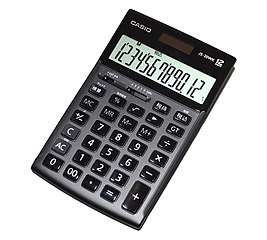
\includegraphics[scale=.63]{DeskCalculator.jpg}\qquad
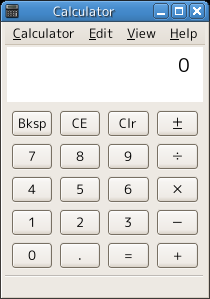
\includegraphics[scale=.5]{Gcalc.png}\qquad\qquad
\caption{물리적 탁상용 계산기와 소프트웨어 탁상용 계산기\\
         {\scriptsize(이미지 출처: 위키미디어 공용)}}
\end{figure}


이 절에서 지금까지 살펴본 바와 같이 하나의 대상 언어에 지시적 의미구조를
여러가지로 정의하는 것이 가능하며 또 유용하다. 다만 이런 의미구조들끼리
서로 호환되는지, 기준으로 삼을 만한 가장 원론적인 의미구조와 비교해
어긋나는 부분은 없는지 물샐틈없이 엄밀하게 논리적으로 증명할 필요성이 있다.
활용 목적에 따라 편리한 대로만 정의한다면 모양새 혹은
문법구조만 같을 뿐 의미가 호환되지 않아 실제로는 다른 언어를 표현하면서도
서로 같은 언어를 다룬다고 착각하게 될지도 모르기 때문이다. 이 책의 내용을
엄밀한 이론적 기술을 강조하는 방향으로 구성하지 않았으므로 그런 증명까지
다루지 않겠지만 확실하게 짚고 넘어가야 하는 중요한 사안이라는 점에 대해서는
재차 강조하고 싶다. 이 장에서 다루는 정규식과 관련한 더 자세한 이론적
성질의 증명에 관해서는 계산이론이나 오토마타이론을 다루는
교재\cite{Sipser2013,Hopcroft2007}를, 그 외의 프로그래밍언어 일반에
활용되는 논리적 방법론을 소개하는 내용으로는 \citet{PFPL2nd}의 교재를
참고하라.


\section{동작방식 의미구조}
동작방식 의미구조(operational semantics)는
프로그램의 의미를 수학적 구조 등 외부의 대상에 지시함으로써 찾는 것이
아니라 프로그램이 계산되는 과정 자체를 프로그램의 의미로 삼는 방식의
의미구조를 말한다. 철학적으로는 의미가 대상에 내재된 것이 아니라 대상들의
관계 속에서 찾아야 한다는 구조주의적 관점과 일맥상통하는 측면이 있다.
참고로 구조주의는 (자연)언어를 기호(sign)의 체계(system), 즉 기호들의
상호관계에 기반한 구조로 이해해야 한다는 소쉬르\cite{Saussure1916}의
언어철학적 관점에서 그 기원을 찾을 수 있다.

\begin{figure}\centering
\begin{subfigure}{.2\textwidth}
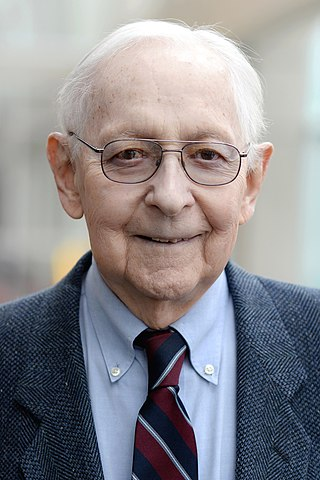
\includegraphics[trim={0 50pt 0 0},clip]{JanuszBrzozowski.jpg}
\end{subfigure}
\begin{subfigure}{.6\textwidth}
언어 $L\subset\Sigma^{*}$의 문자열 $x\in\Sigma$에 대한\\[1.1ex]
브쇼조브스키 미분(Brzozowski derivative):
\[ x^{-1} L ~=~ \{\,y \mid xy\in L\,\} \]

\end{subfigure}
\caption{야누스 브쇼조브스키(Janusz Brzozowski)가 연구한 \\
         언어의 문자열에 대한 미분
         {\scriptsize(사진 출처: 위키미디어 공용)}
         \label{fig:Brzozowski}}
\end{figure}



\lipsum[]

\section{공리적 의미구조}
공리적 의미구조(axiomatic semantics)에 대해서는 이 책에서는 많이
다루지 않으므로 간략히 개념만 설명하고 넘어가겠다. 그렇다고 해서
그다지 중요하지 않은 프로그래밍언어의 의미구조 표현 방식이라는 뜻은
결코 아니다. 어떤 관점에서는 공리적 의미구조야말로 지금까지 실용적
활용 사례\footnote{단적으로, NASA에서도 활용한다.
  \url{https://ti.arc.nasa.gov/tech/rse/publications/vnv/}}가 가장 많은
의미구조의 표현 방식이라 볼 수도 있다. 역사적으로도 공리적 의미구조의
기원이 되는 이론인 호어 논리(Hoare logic)\cite{Hoare69}의 발표와 함께
프로그램 검증(program verification) 분야가 본격적으로
시작하였다\cite{GSLeeHJKim20Hoare}고 본다. 오늘날에는 호어 논리를
확장한 분리 논리(separation logic)\cite{IshtiaqOHearn01,
OHearnReynoldsYang01}를 프로그램 검증에 활용하는 추세다.

% \begin{figure}
% \includegraphics[]{Hoare}
% \caption{Sir Charles Antony Richard Hoare \label{fig:Hoare}}
% \end{figure}


프로그램 검증은 일반적인 검사(testing) 방식의 한계를 극복할 수 있게 한다.
비유하자면 개미는 모두 검다는 성질을 확인하기 위해 10000마리의 개미를
확인해 보니 모두 검은 개미였다 할지라도 10001번째 잡은 개미가 붉은
개미일 수 있듯이, 프로그램이 어떤 성질을 만족한다는 10000개의 테스트를
통과했더라도 또 다른 10001번째 입력으로 실행했을 때 만족하리라는 보장이
없다는 것이 일반적인 검사 방식의 근본적인 한계이다. 프로그램을 실제로
실행하여 구체적인 입력 사례와 그 결과값을 개별적으로 확인하는 일반적인
검사 방식과 달리, 프로그램을 직접 실행하지 않고 그 설계도인 소스코드로부터
수학에서의 증명처럼 모든 가능한 경우에 대해 프로그램이 원하는 성질을
만족함을 보이는 것을 `프로그램 검증'이라 한다. 여기서 ``원하는 성질''이
어떤 내용인지 분명하고 자세하면서도 정확하게 표현하기 위해 고안된
형식논리(formal logic) 체계가 바로 호어 논리이다. 참고로, 프로그램이
의도한 바대로 동작하기 원하는 성질을 분명하고 자세히 표현했다는 뜻에서
그러한 내용을 `명세'(specification)라 일컫는다. 정리하면, 프로그램이
항상 그 명세(specification)대로 동작할 것임을 소스코드로부터 입증하는
것을 `프로그램 검증'이라 하며 이러한 검증에 활용되는 대표적인 형식논리
체계가 `호어 논리'이다.

호어 논리의 문장(statement)은 $\{P\}\,C\,\{Q\}$ 형태로 작성되는데,
$P$, $C$, $Q$의 세 요소로 구성되므로 호어 트리플(Hoare triple)이라고도
부른다. $C$는 명세의 대상이 되는 프로그래밍 언어의 문장(statement) 혹은
명령(command)이며, 명세의 내용에 해당하는 ${P}$와 ${Q}$를 각각
전제조건(precondition)과 사후조건(postcondition)이라 한다.
참고로, $C$의 실행에 앞서 만족되어 있어야 할 조건인 $P$와
실행 이후에 만족되어야 할 할 조건인 $Q$를 그런 의미에서
선행조건(precondition)과 후행조건(postcondition)으로 옮기기도 한다.
실제 프로그램 소스코드보다 일상생활에서 친숙한 내용을 다음과 같은
호어 트리플로 작성해 볼 수 있다.
\begin{quote}\small
\{밥 $n+1$공기 이상 있음\}\;``밥\;1공기\;먹어''\;\{밥 $n$공기 이상 있음\}
~~(단, $n\ge 0$)
\end{quote}
이렇게 선행조건과 후행조건으로 기본적인 명령의 의미구조를 나타내는데,
위의 호어 트리플은 증명해야 할 대상이 아닌 형식논리 체계에서
받아들여야 하는 공리(axiom)로서의 역할을 하기 때문에 이러한 방식으로
프로그래밍언어의 의미구조를 정의하는 것을 `공리적 의미구조'라
일컫는다. 위에서 $n$은 하나의 값으로 정해진 것이 아니라 해당 명령을
사용하는 사례마다 적절히 다른 값으로 구체화할 수 있다. 그러니까 하나로
정해진 공리(axiom)가 아닌 여러 공리를 대표하는 일반적인 공리의 형태를
나타낸다는 뜻에서 공리꼴(axiom schema) 혹은 공리 도식이라고 일컫는다.

(명령형) 프로그래밍 언어에서는 여러 문장을 연달아 작성하여 차례대로
실행할 수 있다. 달리 말하자면 명령 $C_1$과 $C_2$를 순차적으로 실행하라는
복합적 명령 $C_1;C_2$를 작성할 수 있다는 이야기다. 따라서 밥 한 공기
먹고 나서 밥을 또 한 공기 먹는 복합적 명령은 다음과 같이 작성하면 된다.
\begin{quote}\small
``밥 1공기 먹어'';``디저트 1그릇 먹어''
\end{quote}
호어 논리에는 이런 복합적 명령에 대한 명세를 다루는 데 유용한
다음의 추론 규칙이 제공된다.
\begin{quote}
\( \inference[composition]{ \{P\}C_1\{R\} & \{R\}C_2\{Q\} }{
                            \{P\}\,C_1;C_2\,\{Q\} } \)
\end{quote}
먼저 실행되는 $C_1$의 후행조건과 다음에 실행되는 $C_2$의 선행조건이
$R$로 일치할 경우 두 명령을 조합(composition)한 $C_1;C_2$에 대한
호어 트리플을 구성할 수 있음을 말한다.

방금 위에서 소개한 규칙에 따라 밥 한 공기 먹고 또 한 공기 더
먹는 복합명령에 대한 호어 트리플을 구성해 보자. 우선 우리가
앞서 살펴본 호어 트리플을, 내용이 길어지므로 이제부터
좀 더 간략한 표기로, 나란히 써놓고 살펴보자.
\begin{quote}\small
$\{\text{밥}\ge n'+1\}\,\text{``밥\,1\,먹어''}\,\{\underline{\text{밥}\ge n'}\}$
\qquad
$\{\underline{\text{밥}\ge n+1}\}\,\text{``밥\,1\,먹어''}\,\{\text{밥}\ge n\}$
\end{quote}
왼쪽과 오른쪽 호어 트리플에서 $n$값이 서로 다를 수 있으므로 한쪽을 $n'$로
구분하였다. 조합(composition) 규칙을 적용하려면 밑줄 친 왼쪽 명령의
후행조건과 오른쪽 명령의 선행조건이 일치해야 하므로, 왼쪽의 $n'$를
$n+1$로 구체화하여 일치시킨 후 아래와 같이 추론 가능하다.
{\small
\[
\inference[]{
  \{\text{밥}\ge (n+1)+1\}\,\text{``밥\,1\,먹어''}\,\{\text{밥}\ge n+1\}
  &
  \{\text{밥}\ge n+1\}\,\text{``밥\,1\,먹어''}\,\{\text{밥}\ge n\}
}{
  \{\text{밥}\ge (n+1)+1\}
  \,\text{``밥\,1\,먹어''};\text{``밥\,1\,먹어''}\,
  \{\text{밥}\ge n\}
}
\]
}
이렇게 복합명령에 대한 호어 트리플 {\small
$\{\text{밥}\ge n+2\}
 \,\text{``밥\,1\,먹어''};\text{``밥\,1\,먹어''}\,
 \{\text{밥}\ge n\}$}을 공리꼴로부터 추론 규칙을 활용해
유도할 수 있음을 살펴보았다. 참고로, 호어 논리에는 연달아 실행하는
순차적 복합문 외에도 (명령형) 프로그래밍언어에 공통적으로 나타나는
조건문과 반복문에 대한 추론규칙들도 추가로 제공된다. 그런 추론 규칙들을
활용하면 공리꼴부터 다양한 프로그램에 대한 공리적 의미구조에 해당하는
호어 트리플을 도출할 수 있다.

지금까지 공리적 의미구조의 기본적인 개념을 다소 피상적인 비유를 통해
최대한 간단히 표면적으로나마 살펴보았다. 이런 공리적 의미구조가
프로그램 검증에 많이 활용되는 까닭은 프로그램 검증 분야의 초기부터
역사를 함께했다는 이유도 있지만 호어 로직 방식 명세의 유연함이라는
장점 또한 하나의 요인이 된다. 호어 트리플의 선행조건과 후행조건을
명세하는 구체적인 형식논리체계는 검증하고자 하는 성질에 적합한 것으로
선택할 수 있다. 또한 프로그램의 모든 의미를 포괄할 필요 없이 집중하고자
하는 성질에 대해서만 명세하고 나머지를 생략하는 것도 얼마든지 가능하다.
예컨대, 메모리를 얼마나 사용하는지 중점적으로 검증할 때에는 계산되는
대부분의 결과값을 무시하고 얼마나 많은 변수가 선언되고 메모리 할당이
일어났는지만을 중심으로 공리적 의미구조를 정의하는 것이 가능하며,
구현된 알고리즘의 복잡도와 관련된 개념을 검증하고자 할 때는
이를테면 비교 연산이나 산술 연산 등 핵심 연산이 얼마나 많이
수행되는지에만 집중하여 표현된 공리적 의미구조를 정의하는 것도 가능하다.

\section*{요점정리}
\begin{itemize}
 \item TODO TODO TODO TODO TODO TODO TODO TODO TODO TODO TODO TODO
 \item TODO TODO TODO TODO TODO TODO TODO TODO TODO TODO TODO TODO
 \item TODO TODO TODO TODO TODO TODO TODO TODO TODO TODO TODO TODO
\end{itemize}

\section*{연습문제}
\begin{enumerate}
 \item TODO TODO TODO TODO TODO TODO TODO TODO TODO TODO TODO TODO
 \item TODO TODO TODO TODO TODO TODO TODO TODO TODO TODO TODO TODO
 \item TODO TODO TODO TODO TODO TODO TODO TODO TODO TODO TODO TODO
\end{enumerate}

\section*{탐구과제}
\begin{enumerate}
 \item TODO TODO TODO TODO TODO TODO TODO TODO TODO TODO TODO TODO
 \item TODO TODO TODO TODO TODO TODO TODO TODO TODO TODO TODO TODO
 \item TODO TODO TODO TODO TODO TODO TODO TODO TODO TODO TODO TODO
\end{enumerate}

\part{파트}

\chapter{첫째장 제목}
TODO TODO TODO TODO TODO TODO TODO TODO TODO TODO TODO TODO
TODO TODO TODO TODO TODO TODO TODO TODO TODO TODO TODO TODO
TODO TODO TODO TODO TODO TODO TODO TODO TODO TODO TODO TODO

%%%%%%%%%%%%%%%%%%%%%%%%%%%%%%%%%%%%%%%%%%%%%%%%%%%%%%
\printbibliography[title=참고문헌]

\end{document}
